\documentclass[11pt,a4paper]{article}

% --- Packages (identical to main.tex) ---
\usepackage[utf8]{inputenc}
\usepackage[margin=1in]{geometry}
\usepackage[breaklinks=true,colorlinks,citecolor=blue,linkcolor=blue,urlcolor=blue]{hyperref}
\usepackage[table,xcdraw]{xcolor}
\usepackage{epsfig, mathrsfs, latexsym, subfigure, marginnote, gensymb, amsmath}
\usepackage{graphicx}
\usepackage{booktabs}
\usepackage{adjustbox}
\usepackage{doi}

% Package to handle multiple authors and affiliations cleanly in the article class
\usepackage{authblk}

% --- Supporting-information numbering: S1, Table S1, Figure S1 ---
\renewcommand{\thesection}{S\arabic{section}}
\renewcommand{\thetable}{S\arabic{table}}
\renewcommand{\thefigure}{S\arabic{figure}}
\renewcommand{\theequation}{S\arabic{equation}}

% --- Metadata ---
\title{\textbf{Supporting Information for: pydemi: A Dual-Input Python Framework for Charge-Density-Derived Materials Descriptors via DFT and Machine Learning}}

\author[1]{Shubham Kumar Maurya}
\author[1]{Somnath Bhowmick\thanks{bsomnath@iitk.ac.in}}
\affil[1]{Department of Materials Science \& Engineering, Indian Institute of Technology Kanpur, Kanpur 208016, India}

\date{\today}

\begin{document}

\maketitle

\noindent Every number in this document is produced by the scripts in
\texttt{paper/analysis/} and \texttt{docs/*/scripts/} of the pydemi repository;
the full per-family reports, with all their tables and figures, are in
\texttt{docs/}. Section numbers of the main text are referred to as
``main text, Section~$n$''.

\tableofcontents

% ==========================================================================
\section{Descriptor catalogue}
\label{sec:si-catalogue}

Tables~\ref{tab:si-catalogue}--\ref{tab:si-magpie} list every descriptor of the
current release. They are generated from the registry
(\texttt{tools/generate\_docs.py} writes \texttt{docs/catalogue.csv};
\texttt{paper/analysis/k\_si\_tables.py} formats it), so the formulas are the
docstrings the code is registered with. The five domains contain 88
non-compositional descriptors and 132 adopted compositional ones; the
off-by-default \texttt{paw} extension adds 12 and the \texttt{robust}
extension one. Every descriptor is intensive; degenerate cases return the
documented sentinel value together with a \texttt{<name>\_\_flag} column,
never a bare NaN (except \texttt{*\_within\_element\_var} when no element has
two sites, which is flagged and accompanied by the per-element site counts).

\begin{table}[p]
\centering
\caption{Descriptor catalogue (part 1 of 3): every non-compositional descriptor of the registry, generated from \texttt{docs/catalogue.csv}. Domain: b bonding, s structural, m magnetic, h heterogeneity; extension: paw or robust (off by default). Sentinels are the documented values of degenerate cases; stability: r robust, f fragile.}
\label{tab:si-catalogue}
\scriptsize
\begin{tabular}{p{3.3cm}cp{1.4cm}p{6.6cm}p{2.3cm}c}
\toprule
Name & Dom. & Units & Formula & Sentinels & Stab. \\
\midrule
\texttt{zeta} & b & -- & \texttt{1 - sum\_k |grad rho\_k . u\_k| / sum\_k |grad rho\_k|} & uniform\_density=0.0 & r \\
\texttt{m1} & b & \AA & \texttt{sum\_k rho\_k r\_k / sum\_k rho\_k} & zero\_density=0.0 & r \\
\texttt{m2} & b & \AA$^2$ & \texttt{sum\_k rho\_k r\_k\^{}2 / sum\_k rho\_k} & zero\_density=0.0 & r \\
\texttt{sigma\_r2} & b & \AA$^2$ & \texttt{m2 - m1\^{}2} & zero\_density=0.0 & r \\
\texttt{f\_core} & b & -- & \texttt{sum\_\{k: r <= c1\} rho\_k / sum\_k rho\_k} & zero\_density=0.0 & r \\
\texttt{f\_bond} & b & -- & \texttt{sum\_\{k: c1 < r <= c2\} rho\_k / sum\_k rho\_k} & zero\_density=0.0 & r \\
\texttt{f\_int} & b & -- & \texttt{sum\_\{k: r > c2\} rho\_k / sum\_k rho\_k} & zero\_density=0.0 & r \\
\texttt{lnf} & b & -- & \texttt{(1/N) sum\_k 1(lap rho\_k < 0)} & uniform\_density=0.0 & r \\
\texttt{lnf\_charge\_weighted} & b & -- & \texttt{sum\_\{lap rho\_k < 0\} rho\_k / sum\_k rho\_k} & uniform\_density=0.0; zero\_density=0.0 & r \\
\texttt{lap\_concentration} & b & -- & \texttt{sum\_\{lap rho < 0\} |lap rho\_k| / sum\_k |lap rho\_k|} & uniform\_density=0.5 & r \\
\texttt{lap\_concentration\_valence} & b & -- & \texttt{sum\_\{r > c1, lap rho < 0\} |lap rho\_k| / sum\_\{r > c1\} |lap rho\_k|} & uniform\_density=0.5; empty\_region=0.5 & r \\
\texttt{ellip\_bond\_avg} & b & -- & \texttt{mean of lambda1/lambda2 - 1 over \{k in bond, lambda2 < 0\}} & no\_bond\_voxels=0.0 & f \\
\texttt{ellip\_bond\_std} & b & -- & \texttt{std of lambda1/lambda2 - 1 over \{k in bond, lambda2 < 0\}} & no\_bond\_voxels=0.0 & f \\
\texttt{f\_H\_negative} & b & -- & \texttt{(1/N\_bond) sum\_\{k in bond\} 1(H\_k < 0),  H = g + v} & empty\_region=0.0 & r \\
\texttt{H\_bond\_mean} & b & Ha\,bohr$^{-3}$ & \texttt{<H\_k> over the bond shell,  H = g + v = (1/4) lap rho - g (a.u.)} & empty\_region=0.0 & r \\
\texttt{G\_over\_rho} & b & Ha/e & \texttt{<g\_k / rho\_k> over the bond shell (a.u.)} & empty\_region=0.0 & r \\
\texttt{f\_ELF\_localized} & b & -- & \texttt{(1/N\_bond) sum\_\{k in bond\} 1(ELF\_k > 0.5)} & empty\_region=0.0 & r \\
\texttt{ELF\_bond\_avg} & b & -- & \texttt{<ELF\_k> over the bond shell} & empty\_region=0.0 & r \\
\texttt{ELF\_core\_valence\_contrast} & b & -- & \texttt{<ELF>\_core / <ELF>\_bond} & empty\_region=0.0; zero\_denominator=0.0 & r \\
\texttt{zeta\_ELF} & b & -- & \texttt{1 - sum\_k |grad ELF\_k . u\_k| / sum\_k |grad ELF\_k|} & uniform\_density=0.0 & r \\
\texttt{f\_NCI} & b & -- & \texttt{(1/N) sum\_k 1(s\_k < 0.5 and rho\_k < 0.05 a.u.),  s = |grad rho| / (2 (3 pi\^{}2)\^{}(1/3) rho\^{}(4/3))} & uniform\_density=0.0 & r \\
\texttt{NCI\_attractive} & b & -- & \texttt{fraction of NCI voxels with lambda2 < 0} & uniform\_density=0.0; no\_nci\_voxels=0.0 & r \\
\texttt{sign\_lambda2\_rho\_mean} & b & e\,bohr$^{-3}$ & \texttt{mean of sign(lambda2) rho\_k over NCI voxels (rho in a.u.)} & uniform\_density=0.0; no\_nci\_voxels=0.0 & r \\
\texttt{V\_spread} & b & eV & \texttt{std over sites i of V(R\_i)} & -- & r \\
\texttt{V\_int\_min} & b & eV & \texttt{min over interstitial voxels of V\_k (cell average of V set to 0)} & empty\_region=0.0 & r \\
\texttt{rho\_mid\_mean} & b & e\,\AA$^{-3}$ & \texttt{mean of rho at nearest-neighbour bond midpoints} & no\_bonds=0.0 & r \\
\texttt{rho\_mid\_std} & b & e\,\AA$^{-3}$ & \texttt{std of rho at nearest-neighbour bond midpoints} & no\_bonds=0.0 & r \\
\texttt{m1\_def} & b & \AA & \texttt{sum\_k |drho\_k| r\_k / sum\_k |drho\_k|,  drho = rho - promolecule} & zero\_deformation=0.0 & r \\
\texttt{m2\_def} & b & \AA$^2$ & \texttt{sum\_k |drho\_k| r\_k\^{}2 / sum\_k |drho\_k|} & zero\_deformation=0.0 & r \\
\texttt{sigma\_r2\_def} & b & \AA$^2$ & \texttt{m2\_def - m1\_def\^{}2} & zero\_deformation=0.0 & r \\
\texttt{f\_bond\_def} & b & -- & \texttt{sum\_\{k in bond, drho > 0\} drho\_k / sum\_\{drho > 0\} drho\_k} & no\_accumulation=0.0 & r \\
\texttt{f\_int\_def} & b & -- & \texttt{sum\_\{k in int, drho > 0\} drho\_k / sum\_\{drho > 0\} drho\_k} & no\_accumulation=0.0 & r \\
\texttt{f\_bond\_dep} & b & -- & \texttt{sum\_\{k in bond, drho < 0\} |drho\_k| / sum\_\{drho < 0\} |drho\_k|} & no\_depletion=0.0 & r \\
\texttt{def\_polarity} & b & -- & \texttt{sum\_k |drho\_k| dV / Q\_tot,  Q\_tot = sum\_k rho\_k dV} & zero\_density=0.0 & r \\
\bottomrule
\end{tabular}
\end{table}

\begin{table}[p]
\centering
\caption{Descriptor catalogue (part 2 of 3): every non-compositional descriptor of the registry, generated from \texttt{docs/catalogue.csv}. Domain: b bonding, s structural, m magnetic, h heterogeneity; extension: paw or robust (off by default). Sentinels are the documented values of degenerate cases; stability: r robust, f fragile.}
\scriptsize
\begin{tabular}{p{3.3cm}cp{1.4cm}p{6.6cm}p{2.3cm}c}
\toprule
Name & Dom. & Units & Formula & Sentinels & Stab. \\
\midrule
\texttt{bond\_charge\_transfer\_pair\_mean} & b & electrons & \texttt{mean over nearest-neighbour pairs of int\_\{region(i,j)\} drho dV} & no\_bonds=0.0 & r \\
\texttt{bond\_charge\_transfer\_pair\_std} & b & electrons & \texttt{std over nearest-neighbour pairs of int\_\{region(i,j)\} drho dV} & no\_bonds=0.0 & r \\
\texttt{rho\_perc\_a} & s & e\,\AA$^{-3}$ & \texttt{max \{c : the super-level set \{rho > c\} spans a1 under PBC\}} & -- & r \\
\texttt{rho\_perc\_b} & s & e\,\AA$^{-3}$ & \texttt{max \{c : the super-level set \{rho > c\} spans a2 under PBC\}} & -- & r \\
\texttt{rho\_perc\_c} & s & e\,\AA$^{-3}$ & \texttt{max \{c : the super-level set \{rho > c\} spans a3 under PBC\}} & -- & r \\
\texttt{perc\_anisotropy} & s & -- & \texttt{(max\_alpha - min\_alpha) / mean\_alpha of rho\_perc} & zero\_levels=0.0 & r \\
\texttt{n\_max} & s & \AA$^{-3}$ & \texttt{(number of local maxima) / V\_cell} & -- & r \\
\texttt{n\_min} & s & \AA$^{-3}$ & \texttt{(number of local minima) / V\_cell} & -- & r \\
\texttt{n\_saddle1} & s & \AA$^{-3}$ & \texttt{(number of index-1 saddles) / V\_cell} & -- & f \\
\texttt{n\_saddle2} & s & \AA$^{-3}$ & \texttt{(number of index-2 saddles) / V\_cell} & -- & f \\
\texttt{n\_NNM} & s & \AA$^{-3}$ & \texttt{(number of local maxima with min\_i |r - R\_i| > r\_cut) / V\_cell} & -- & r \\
\texttt{Q\_NNM} & s & -- & \texttt{(charge in the steepest-ascent basins of the non-nuclear maxima) / Q\_tot} & -- & r \\
\texttt{rho\_min} & s & e\,\AA$^{-3}$ & \texttt{min\_k rho\_k} & -- & r \\
\texttt{rho\_min\_ratio} & s & -- & \texttt{rho\_min / <rho>\_V} & zero\_density=0.0 & r \\
\texttt{rho\_int\_mean} & s & e\,\AA$^{-3}$ & \texttt{mean of rho over the interstitial shell (r > c2)} & empty\_region=0.0 & r \\
\texttt{T\_eigenvalues\_t1} & s & -- & \texttt{eigenvalue 1 (ascending, t1 <= t2 <= t3) of T\_ab = sum\_k d\_a rho\_k d\_b rho\_k / sum\_k |grad rho\_k|\^{}2 (trace 1)} & uniform\_density=0.3333333333333333 & r \\
\texttt{T\_eigenvalues\_t2} & s & -- & \texttt{eigenvalue 2 (ascending, t1 <= t2 <= t3) of T\_ab = sum\_k d\_a rho\_k d\_b rho\_k / sum\_k |grad rho\_k|\^{}2 (trace 1)} & uniform\_density=0.3333333333333333 & r \\
\texttt{T\_eigenvalues\_t3} & s & -- & \texttt{eigenvalue 3 (ascending, t1 <= t2 <= t3) of T\_ab = sum\_k d\_a rho\_k d\_b rho\_k / sum\_k |grad rho\_k|\^{}2 (trace 1)} & uniform\_density=0.3333333333333333 & r \\
\texttt{charge\_FA} & s & -- & \texttt{sqrt(3/2) ||T - (1/3) I||\_F / ||T||\_F} & uniform\_density=0.0 & r \\
\texttt{shannon\_entropy} & s & -- & \texttt{-int rho\~{} ln rho\~{} dV - ln V,  rho\~{} = rho / N\_e} & zero\_density=0.0 & r \\
\texttt{fisher\_information} & s & bohr$^{-2}$ & \texttt{int |grad rho\~{}|\^{}2 / rho\~{} dV  (a.u.; voxels above the density floor)} & zero\_density=0.0 & r \\
\texttt{disequilibrium} & s & -- & \texttt{V int rho\~{}\^{}2 dV} & zero\_density=0.0 & r \\
\texttt{LMC\_complexity} & s & -- & \texttt{D e\^{}S  (D, S the unnormalized disequilibrium and entropy; = 1 when uniform)} & zero\_density=0.0 & r \\
\texttt{M\_abs\_per\_atom} & m & $\mu_B$/atom & \texttt{sum\_k |m\_k| dV / n\_atoms} & non\_magnetic=0.0 & r \\
\texttt{M\_net\_per\_atom} & m & $\mu_B$/atom & \texttt{|sum\_k m\_k dV| / n\_atoms} & non\_magnetic=0.0 & r \\
\texttt{m1\_spin} & m & \AA & \texttt{sum\_k |m\_k| r\_k / sum\_k |m\_k|} & non\_magnetic=0.0 & r \\
\texttt{sigma\_r2\_spin} & m & \AA$^2$ & \texttt{sum\_k |m\_k| r\_k\^{}2 / sum\_k |m\_k| - m1\_spin\^{}2} & non\_magnetic=0.0 & r \\
\texttt{f\_bond\_spin} & m & -- & \texttt{sum\_\{k in bond\} |m\_k| / sum\_k |m\_k|} & non\_magnetic=0.0 & r \\
\texttt{mu\_site\_std} & m & $\mu_B$ & \texttt{std over i of mu\_i,  mu\_i = sum\_k w\_i(k) m\_k dV} & non\_magnetic=0.0 & r \\
\texttt{spin\_frustration} & m & -- & \texttt{1 - |sum\_i mu\_i| / sum\_i |mu\_i|} & non\_magnetic=0.0 & r \\
\texttt{spin\_charge\_correlation} & m & -- & \texttt{Pearson r(rho\_k, |m\_k|) over voxels} & non\_magnetic=0.0 & r \\
\texttt{m1\_site\_std} & h & \AA & \texttt{std over sites of X\^{}(i),  X\^{}(i) = sum\_k w\_i(k) rho\_k r\_ik / sum\_k w\_i(k) rho\_k} & uniform\_density=0.0; non\_magnetic=0.0 & r \\
\texttt{m1\_site\_range} & h & \AA & \texttt{max - min over sites of X\^{}(i),  X\^{}(i) = sum\_k w\_i(k) rho\_k r\_ik / sum\_k w\_i(k) rho\_k} & uniform\_density=0.0; non\_magnetic=0.0 & r \\
\texttt{m1\_site\_max} & h & \AA & \texttt{max over sites of X\^{}(i),  X\^{}(i) = sum\_k w\_i(k) rho\_k r\_ik / sum\_k w\_i(k) rho\_k} & uniform\_density=0.0; non\_magnetic=0.0 & r \\
\bottomrule
\end{tabular}
\end{table}

\begin{table}[p]
\centering
\caption{Descriptor catalogue (part 3 of 3): every non-compositional descriptor of the registry, generated from \texttt{docs/catalogue.csv}. Domain: b bonding, s structural, m magnetic, h heterogeneity; extension: paw or robust (off by default). Sentinels are the documented values of degenerate cases; stability: r robust, f fragile.}
\scriptsize
\begin{tabular}{p{3.3cm}cp{1.4cm}p{6.6cm}p{2.3cm}c}
\toprule
Name & Dom. & Units & Formula & Sentinels & Stab. \\
\midrule
\texttt{m1\_site\_min} & h & \AA & \texttt{min over sites of X\^{}(i),  X\^{}(i) = sum\_k w\_i(k) rho\_k r\_ik / sum\_k w\_i(k) rho\_k} & uniform\_density=0.0; non\_magnetic=0.0 & r \\
\texttt{m1\_within\_element\_var} & h & \AA$^2$ & \texttt{sum\_e w\_e Var\_\{i in e\} of X\^{}(i),  X\^{}(i) = sum\_k w\_i(k) rho\_k r\_ik / sum\_k w\_i(k) rho\_k} & uniform\_density=0.0; non\_magnetic=0.0; one\_site\_per\_element=nan & r \\
\texttt{m1\_between\_element\_var} & h & \AA$^2$ & \texttt{sum\_e w\_e (mean\_e - mean)\^{}2 of X\^{}(i),  X\^{}(i) = sum\_k w\_i(k) rho\_k r\_ik / sum\_k w\_i(k) rho\_k} & uniform\_density=0.0; non\_magnetic=0.0; single\_element=0.0 & r \\
\texttt{f\_bond\_site\_std} & h & -- & \texttt{std over sites of X\^{}(i),  X\^{}(i) = sum\_\{c1 < r\_ik <= c2\} w\_i(k) rho\_k / sum\_k w\_i(k) rho\_k} & uniform\_density=0.0; non\_magnetic=0.0 & r \\
\texttt{f\_bond\_site\_range} & h & -- & \texttt{max - min over sites of X\^{}(i),  X\^{}(i) = sum\_\{c1 < r\_ik <= c2\} w\_i(k) rho\_k / sum\_k w\_i(k) rho\_k} & uniform\_density=0.0; non\_magnetic=0.0 & r \\
\texttt{f\_bond\_site\_max} & h & -- & \texttt{max over sites of X\^{}(i),  X\^{}(i) = sum\_\{c1 < r\_ik <= c2\} w\_i(k) rho\_k / sum\_k w\_i(k) rho\_k} & uniform\_density=0.0; non\_magnetic=0.0 & r \\
\texttt{f\_bond\_site\_min} & h & -- & \texttt{min over sites of X\^{}(i),  X\^{}(i) = sum\_\{c1 < r\_ik <= c2\} w\_i(k) rho\_k / sum\_k w\_i(k) rho\_k} & uniform\_density=0.0; non\_magnetic=0.0 & r \\
\texttt{f\_bond\_within\_element\_var} & h & -- & \texttt{sum\_e w\_e Var\_\{i in e\} of X\^{}(i),  X\^{}(i) = sum\_\{c1 < r\_ik <= c2\} w\_i(k) rho\_k / sum\_k w\_i(k) rho\_k} & uniform\_density=0.0; non\_magnetic=0.0; one\_site\_per\_element=nan & r \\
\texttt{f\_bond\_between\_element\_var} & h & -- & \texttt{sum\_e w\_e (mean\_e - mean)\^{}2 of X\^{}(i),  X\^{}(i) = sum\_\{c1 < r\_ik <= c2\} w\_i(k) rho\_k / sum\_k w\_i(k) rho\_k} & uniform\_density=0.0; non\_magnetic=0.0; single\_element=0.0 & r \\
\texttt{zeta\_site\_std} & h & -- & \texttt{std over sites of X\^{}(i),  X\^{}(i) = 1 - sum\_k w\_i(k) |grad rho\_k . u\_ik| / sum\_k w\_i(k) |grad rho\_k|} & uniform\_density=0.0; non\_magnetic=0.0 & r \\
\texttt{zeta\_site\_range} & h & -- & \texttt{max - min over sites of X\^{}(i),  X\^{}(i) = 1 - sum\_k w\_i(k) |grad rho\_k . u\_ik| / sum\_k w\_i(k) |grad rho\_k|} & uniform\_density=0.0; non\_magnetic=0.0 & r \\
\texttt{zeta\_site\_max} & h & -- & \texttt{max over sites of X\^{}(i),  X\^{}(i) = 1 - sum\_k w\_i(k) |grad rho\_k . u\_ik| / sum\_k w\_i(k) |grad rho\_k|} & uniform\_density=0.0; non\_magnetic=0.0 & r \\
\texttt{zeta\_site\_min} & h & -- & \texttt{min over sites of X\^{}(i),  X\^{}(i) = 1 - sum\_k w\_i(k) |grad rho\_k . u\_ik| / sum\_k w\_i(k) |grad rho\_k|} & uniform\_density=0.0; non\_magnetic=0.0 & r \\
\texttt{zeta\_within\_element\_var} & h & -- & \texttt{sum\_e w\_e Var\_\{i in e\} of X\^{}(i),  X\^{}(i) = 1 - sum\_k w\_i(k) |grad rho\_k . u\_ik| / sum\_k w\_i(k) |grad rho\_k|} & uniform\_density=0.0; non\_magnetic=0.0; one\_site\_per\_element=nan & r \\
\texttt{zeta\_between\_element\_var} & h & -- & \texttt{sum\_e w\_e (mean\_e - mean)\^{}2 of X\^{}(i),  X\^{}(i) = 1 - sum\_k w\_i(k) |grad rho\_k . u\_ik| / sum\_k w\_i(k) |grad rho\_k|} & uniform\_density=0.0; non\_magnetic=0.0; single\_element=0.0 & r \\
\texttt{mu\_site\_range} & h & $\mu_B$ & \texttt{max - min over sites of X\^{}(i),  X\^{}(i) = mu\_i = sum\_k w\_i(k) m\_k dV (signed; |mu\_i| for non-collinear runs)} & uniform\_density=0.0; non\_magnetic=0.0 & r \\
\texttt{mu\_site\_max} & h & $\mu_B$ & \texttt{max over sites of X\^{}(i),  X\^{}(i) = mu\_i = sum\_k w\_i(k) m\_k dV (signed; |mu\_i| for non-collinear runs)} & uniform\_density=0.0; non\_magnetic=0.0 & r \\
\texttt{mu\_site\_min} & h & $\mu_B$ & \texttt{min over sites of X\^{}(i),  X\^{}(i) = mu\_i = sum\_k w\_i(k) m\_k dV (signed; |mu\_i| for non-collinear runs)} & uniform\_density=0.0; non\_magnetic=0.0 & r \\
\texttt{mu\_within\_element\_var} & h & $\mu_B^2$ & \texttt{sum\_e w\_e Var\_\{i in e\} of X\^{}(i),  X\^{}(i) = mu\_i = sum\_k w\_i(k) m\_k dV (signed; |mu\_i| for non-collinear runs)} & uniform\_density=0.0; non\_magnetic=0.0; one\_site\_per\_element=nan & r \\
\texttt{mu\_between\_element\_var} & h & $\mu_B^2$ & \texttt{sum\_e w\_e (mean\_e - mean)\^{}2 of X\^{}(i),  X\^{}(i) = mu\_i = sum\_k w\_i(k) m\_k dV (signed; |mu\_i| for non-collinear runs)} & uniform\_density=0.0; non\_magnetic=0.0; single\_element=0.0 & r \\
\texttt{m1\_def\_out} & b (paw) & \AA & \texttt{sum |drho\_k| r\_k / sum |drho\_k| over voxels outside every PAW augmentation sphere (r > R\_PAW of the nearest nucleus)} & empty\_region=0.0; zero\_deformation=0.0 & r \\
\texttt{m2\_def\_out} & b (paw) & \AA$^2$ & \texttt{sum |drho\_k| r\_k\^{}2 / sum |drho\_k| over voxels outside every PAW augmentation sphere (r > R\_PAW of the nearest nucleus)} & empty\_region=0.0; zero\_deformation=0.0 & r \\
\texttt{sigma\_r2\_def\_out} & b (paw) & \AA$^2$ & \texttt{m2\_def\_out - m1\_def\_out\^{}2 over voxels outside every PAW augmentation sphere (r > R\_PAW of the nearest nucleus)} & empty\_region=0.0; zero\_deformation=0.0 & r \\
\texttt{f\_bond\_def\_out} & b (paw) & -- & \texttt{sum\_\{bond, drho > 0\} drho / sum\_\{drho > 0\} drho over voxels outside every PAW augmentation sphere (r > R\_PAW of the nearest nucleus)} & empty\_region=0.0; no\_accumulation=0.0 & r \\
\texttt{f\_int\_def\_out} & b (paw) & -- & \texttt{sum\_\{int, drho > 0\} drho / sum\_\{drho > 0\} drho over voxels outside every PAW augmentation sphere (r > R\_PAW of the nearest nucleus)} & empty\_region=0.0; no\_accumulation=0.0 & r \\
\texttt{f\_bond\_dep\_out} & b (paw) & -- & \texttt{sum\_\{bond, drho < 0\} |drho| / sum\_\{drho < 0\} |drho| over voxels outside every PAW augmentation sphere (r > R\_PAW of the nearest nucleus)} & empty\_region=0.0; no\_depletion=0.0 & r \\
\texttt{def\_polarity\_out} & b (paw) & -- & \texttt{sum |drho\_k| dV / Q\_tot over voxels outside every PAW augmentation sphere (r > R\_PAW of the nearest nucleus)} & empty\_region=0.0; zero\_density=0.0 & r \\
\texttt{def\_out\_volume\_fraction} & b (paw) & -- & \texttt{fraction of the cell outside every PAW augmentation sphere} & -- & r \\
\texttt{rho\_min\_int} & s (paw) & e\,\AA$^{-3}$ & \texttt{min of rho over voxels with r > max(c2, R\_PAW) of their nearest nucleus} & empty\_region=0.0 & r \\
\texttt{rho\_min\_int\_ratio} & s (paw) & -- & \texttt{rho\_min\_int / <rho>\_V} & empty\_region=0.0; zero\_density=0.0 & r \\
\texttt{n\_NNM\_paw} & s (paw) & \AA$^{-3}$ & \texttt{(number of local maxima with r > max(r\_cut, R\_PAW,i)) / V\_cell} & -- & r \\
\texttt{Q\_NNM\_paw} & s (paw) & -- & \texttt{(charge in the basins of the maxima counted by n\_NNM\_paw) / Q\_tot} & -- & r \\
\texttt{ellip\_bond\_bounded\_avg} & b (robust) & -- & \texttt{mean of 1 - lambda2/lambda1 over \{k in bond, lambda2 < 0\}} & no\_bond\_voxels=0.0 & r \\
\bottomrule
\end{tabular}
\end{table}

\begin{table}[htbp]
\centering
\caption{The 132 adopted compositional descriptors: matminer's Magpie preset, 44 elemental properties times 6 statistics (\texttt{magpie\_<statistic>\_<property>}), tagged \texttt{adopted=True} in the registry.}
\label{tab:si-magpie}
\small
\begin{tabular}{p{3cm}p{11cm}}
\toprule
Statistics & avg, maximum, mean, minimum, mode, range \\
Properties & AtomicWeight, Column, CovalentRadius, Electronegativity, GSbandgap, GSmagmom, GSvolume\_pa, MeltingT, MendeleevNumber, NUnfilled, NValence, NdUnfilled, NdValence, NfUnfilled, NfValence, NpUnfilled, NpValence, NsUnfilled, NsValence, Number, Row, SpaceGroupNumber, dev\_AtomicWeight, dev\_Column, dev\_CovalentRadius, dev\_Electronegativity, dev\_GSbandgap, dev\_GSmagmom, dev\_GSvolume\_pa, dev\_MeltingT, dev\_MendeleevNumber, dev\_NUnfilled, dev\_NValence, dev\_NdUnfilled, dev\_NdValence, dev\_NfUnfilled, dev\_NfValence, dev\_NpUnfilled, dev\_NpValence, dev\_NsUnfilled, dev\_NsValence, dev\_Number, dev\_Row, dev\_SpaceGroupNumber \\
\bottomrule
\end{tabular}
\end{table}


% ==========================================================================
\section{Numerical details}
\label{sec:si-numerics}

% To be populated when main-text Section 4 is trimmed. The following move here
% in full, with the main text keeping one summary sentence and a pointer each:
%  - S2.1 Derivatives: full scheme comparison (tab:derivatives, all descriptors),
%         the isolated-atom FFT round-off test.
%  - S2.2 Partitions: Becke truncation table (tab:partitions), the full
%         partition-sensitivity table (tab:partition-sensitivity).
%  - S2.3 PAW: negative densities, pseudized nuclei and the NNM_paw cutoff,
%         the FeNi3 shell table (tab:feni3), valence counts and the nine
%         semicore elements, Hirshfeld charges against electronegativity.
%  - S2.4 The critical-point census: the Freudenthal identity, the
%         stencil-dependence of extrema.
%  - S2.5 Grid convergence (all descriptors) and the ellipticity variants
%         (tab:ellipticity).
%  - S2.6 Documented corrections to the specification.

% ==========================================================================
\section{Descriptor families: behaviour on model and real densities}
\label{sec:si-families}

This section condenses the six per-family reports of the repository
(\texttt{docs/anisotropy\_descriptors}, \texttt{deformation\_descriptors},
\texttt{heterogeneity\_descriptors}, \texttt{magnetic\_descriptors},
\texttt{percolation\_descriptors}, \texttt{ionicity\_descriptors}). For each
family it gives the exact tests on model densities, what the descriptors
measure on the 6,059 PAW pseudo-densities, and the resulting caveats. Chemical
classes are assigned by the anions present (elemental, intermetallic,
boride/carbide, hydride, pnictide, chalcogenide, oxide, halide; first match),
crystal systems from the relaxed structures with spglib (tolerance
$10^{-3}$\,\AA).

% --------------------------------------------------------------------------
\subsection{Gradient anisotropy: \texttt{zeta}, \texttt{zeta\_ELF}, \texttt{T\_eigenvalues}, \texttt{charge\_FA}}

For an anisotropic Gaussian $\rho\propto e^{-(ax^2+ay^2+cz^2)}$ the
anisotropy tensor $T_{ab}=\sum\partial_a\rho\,\partial_b\rho/\sum|\nabla\rho|^2$
is exactly $\mathrm{diag}(a,a,c)/(2a+c)$; pydemi reproduces its eigenvalues
and the fractional anisotropy to $10^{-14}$ (Fig.~\ref{fig:si-aniso-analytic}),
and gives $\zeta=0$ and $T=I/3$ for a spherical atom.

On real densities \texttt{charge\_FA} is a symmetry detector: for the 2,137
structures that are cubic after relaxation it is at the numerical floor
(median $4\times10^{-8}$), whereas it exceeds $10^{-3}$ for 69--86\% of every
lower-symmetry crystal system and picks out layered and linear-unit structures
(graphite 0.50, h-BN 0.25, the azides 0.42). Magnetic cubic Yb, Dy and Pr
compounds reach $4\times10^{-3}$: the density breaks the cubic symmetry while
the lattice keeps it. \texttt{zeta} separates covalent from ionic bonding
(Si 0.21, GaAs 0.13; KCl 0.009, Cu 0.003), but the augmentation spheres, 46\%
of the volume, carry 86\% of its denominator
(Fig.~\ref{fig:si-aniso-regions}), so on a CHGCAR it partly measures the
pseudized density near the nuclei. \texttt{zeta\_ELF} is high for electrides
(Ca$_2$N 0.54) but changes by 18--26\% between derivative schemes and has a
baseline of up to 0.24 for a spherical atom, whose exact value is 0.

\begin{figure}[htbp]
\centering
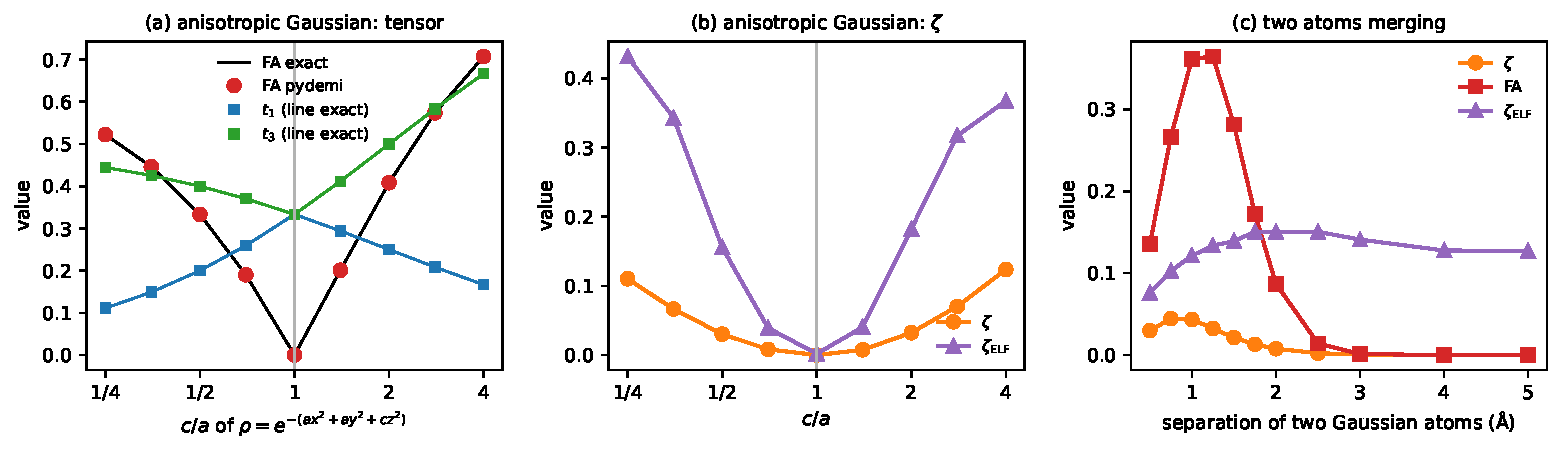
\includegraphics[width=\textwidth]{figures/si/anisotropy_fig01_analytic.pdf}
\caption{Anisotropy descriptors on model densities: (a) an anisotropic Gaussian
against the exact tensor, (b) \texttt{zeta} of the same, (c) two Gaussian atoms
merging.}
\label{fig:si-aniso-analytic}
\end{figure}

\begin{figure}[htbp]
\centering
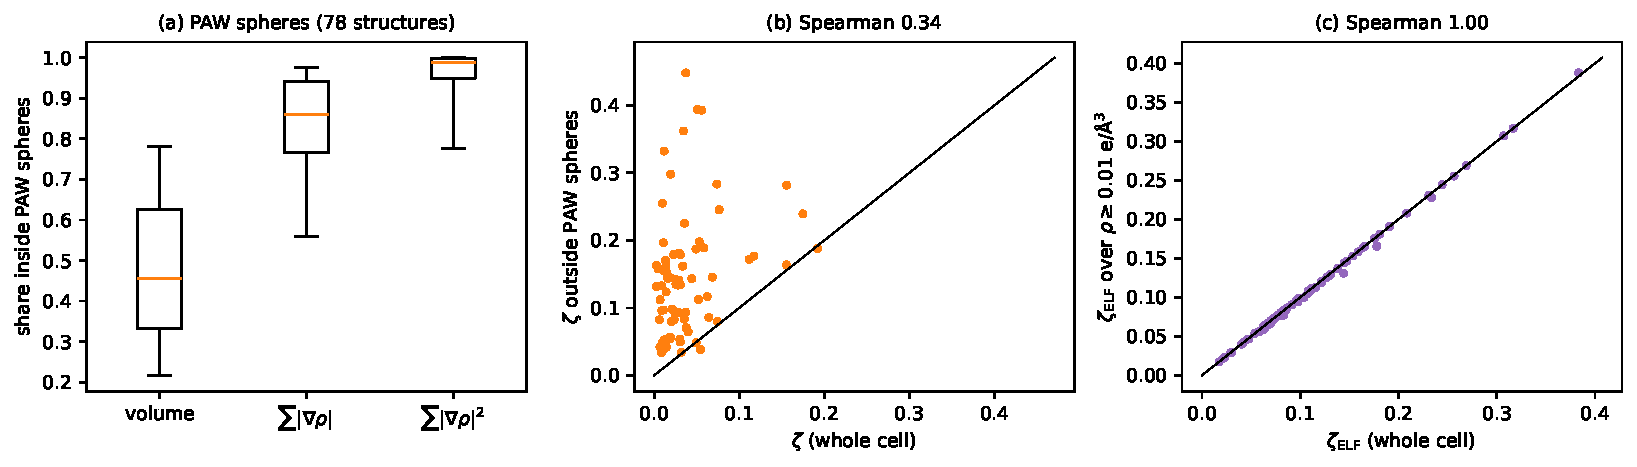
\includegraphics[width=\textwidth]{figures/si/anisotropy_fig11_region_shares.pdf}
\caption{Where the anisotropy sums come from on PAW densities (100 random
structures): share of $\sum|\nabla\rho|$ and $\sum|\nabla\rho|^2$ inside the
augmentation spheres, and \texttt{zeta}, \texttt{charge\_FA} and
\texttt{zeta\_ELF} recomputed outside them.}
\label{fig:si-aniso-regions}
\end{figure}

% --------------------------------------------------------------------------
\subsection{Deformation density: \texttt{m1\_def} \ldots\ \texttt{def\_polarity}}

With a Gaussian ``breathing'' atom against its own reference, all seven
deformation descriptors match one-dimensional radial quadrature to 0.003 or
better. Moving $q$ electrons into a bond or onto a neighbour makes
\texttt{def\_polarity} exactly linear in $q$, while the six shape descriptors
stay constant to $10^{-3}$: they are invariant under $\Delta\rho\to\lambda\Delta\rho$
(Fig.~\ref{fig:si-def-models}). Because the shells are absolute (0.8 and
1.5\,\AA), bond charge of bonds longer than about 3.3\,\AA\ is counted as
interstitial.

None of the 6,059 runs provides AECCAR files, so every deformation density is
the PAW pseudo-density minus tabulated free-atom valence densities. A median
87\% of $\int|\Delta\rho|$ lies inside the augmentation spheres, which fill 48\%
of the volume, and most of the accumulation counted by the shells sits in the
core shell (median 65\%; Fig.~\ref{fig:si-def-paw}). The whole-cell values and
the \texttt{paw}-extension values computed outside the spheres are
statistically unrelated (Spearman 0.00 for \texttt{m1\_def}, $-0.30$ for
\texttt{def\_polarity}); only the latter follow chemistry, e.g.
\texttt{def\_polarity\_out} rises with the electronegativity difference
(Spearman $+0.39$) and \texttt{f\_bond\_def\_out} is 0.91--1.00 for compounds
with anions but about 0.5 for metals (Fig.~\ref{fig:si-def-class}). With a
rule-based instead of the correct valence count the family is destroyed
(median change 55\% for \texttt{def\_polarity}), and \texttt{f\_bond\_def}
depends strongly on the inner shell radius (Spearman 0.25 between $c_1=0.8$
and 0.6\,\AA).

\begin{figure}[htbp]
\centering
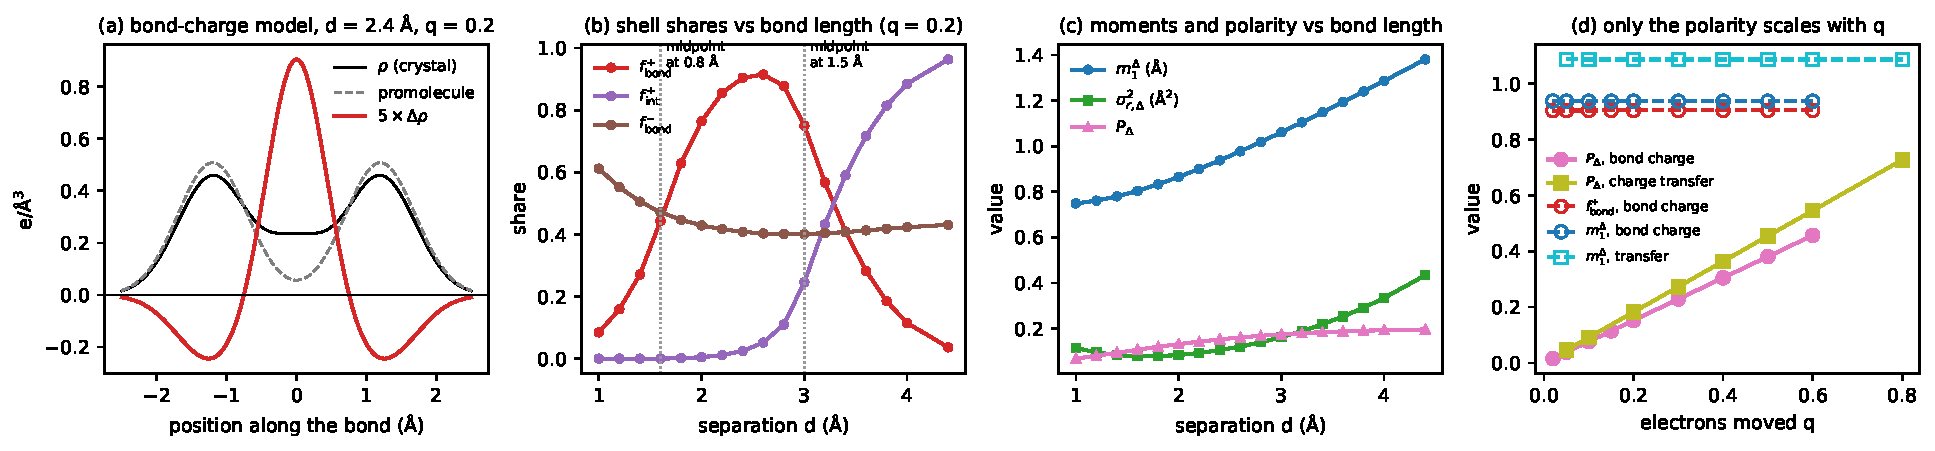
\includegraphics[width=\textwidth]{figures/si/deformation_fig02_bond_charge_models.pdf}
\caption{Bond-charge and charge-transfer models: shell shares against bond
length and the linearity of \texttt{def\_polarity} in the moved charge.}
\label{fig:si-def-models}
\end{figure}

\begin{figure}[htbp]
\centering
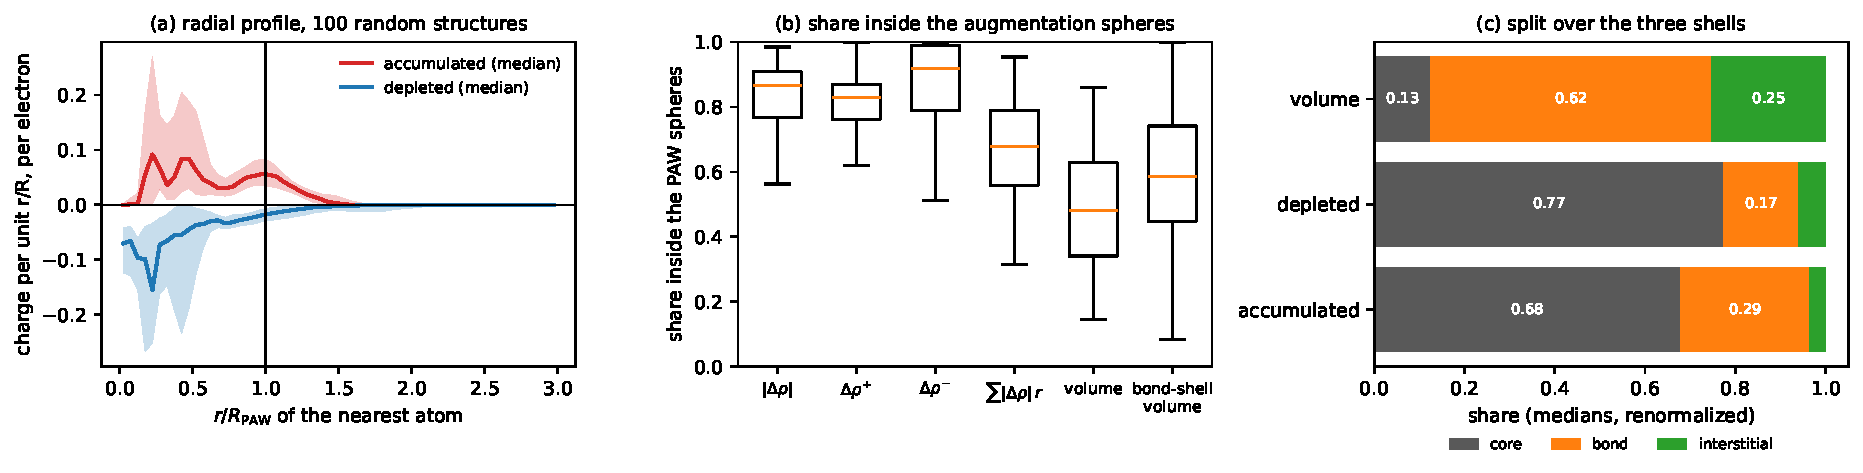
\includegraphics[width=\textwidth]{figures/si/deformation_fig05_paw_dominance.pdf}
\caption{The deformation density of CHGCARs is dominated by the augmentation
spheres (100 random structures): radial profile against $r/R_{\mathrm{PAW}}$,
shares inside the spheres, and the split over the core, bond and interstitial
shells.}
\label{fig:si-def-paw}
\end{figure}

\begin{figure}[htbp]
\centering
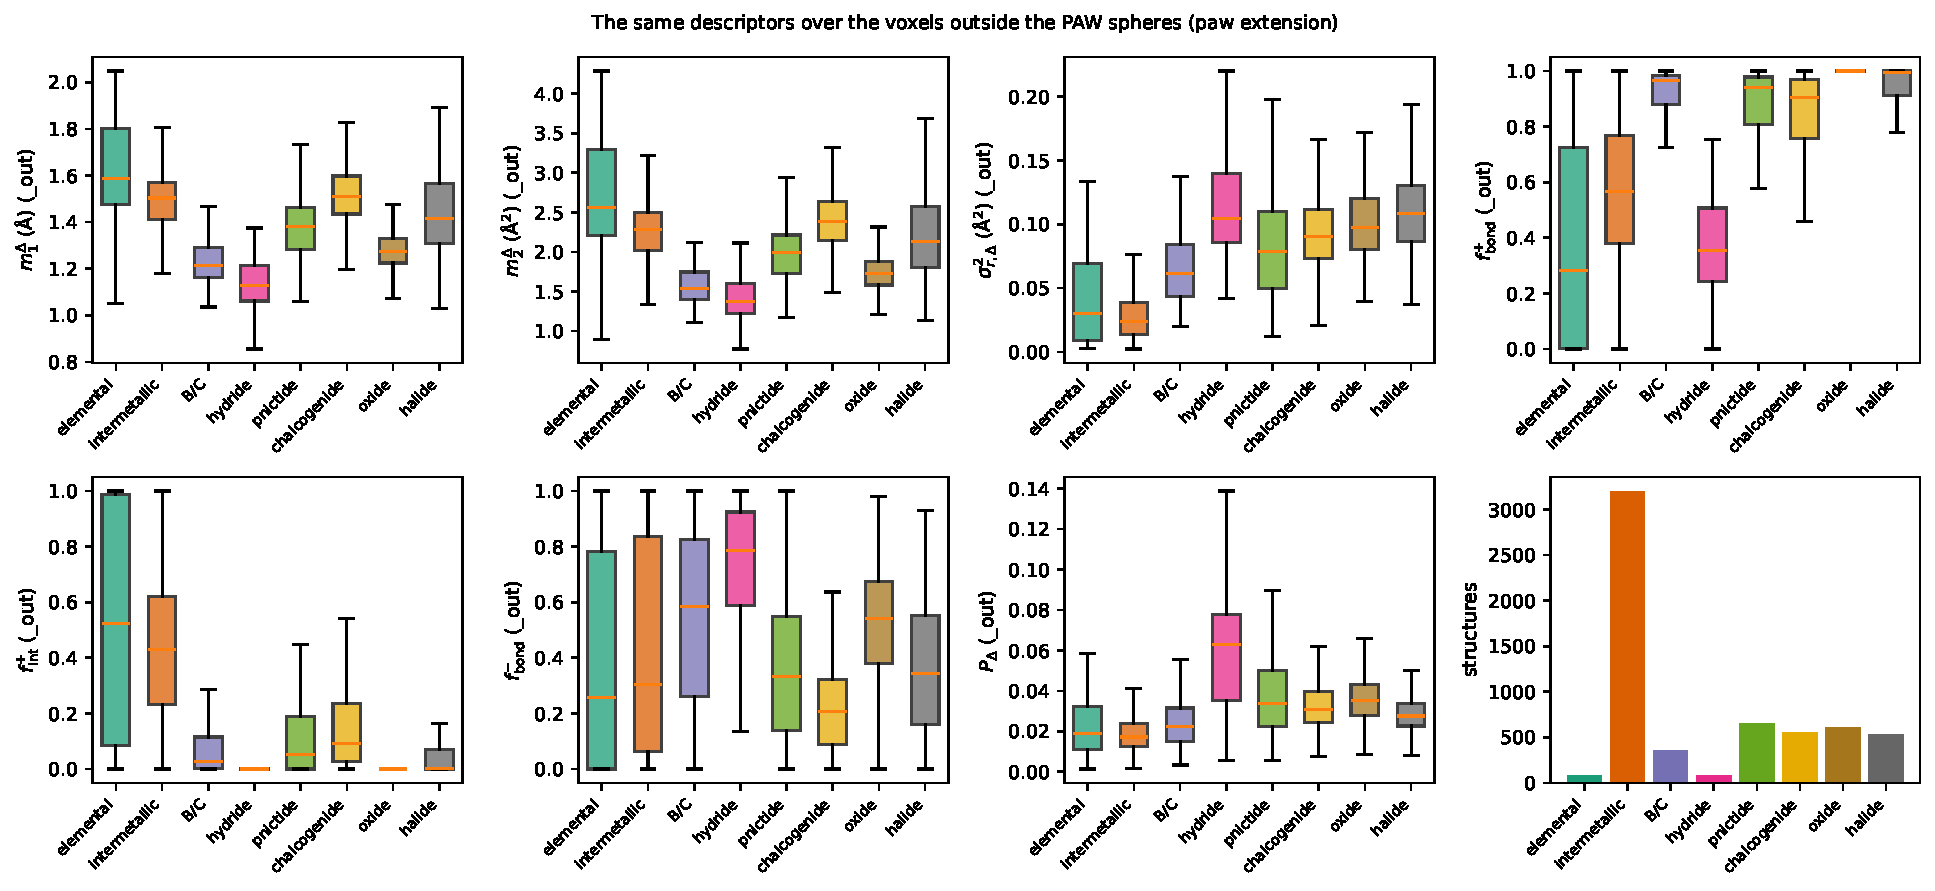
\includegraphics[width=\textwidth]{figures/si/deformation_fig08_by_class_out.pdf}
\caption{Deformation descriptors outside the augmentation spheres
(\texttt{paw} extension) by chemical class.}
\label{fig:si-def-class}
\end{figure}

% --------------------------------------------------------------------------
\subsection{Site heterogeneity: \texttt{*\_site\_std} and the within/between-element variances}

The one-way decomposition $\mathrm{std}^2=\text{within}+\text{between}$ holds to
a relative $10^{-15}$ on all 6,059 structures and $10^{-17}$ on model
crystals. In a rock-salt model where symmetry makes all sites of an element
equivalent the within-element variance is $10^{-29}$; one ``defect'' site makes
it 6--10 times the between-element part, and random displacements make it grow
smoothly (Fig.~\ref{fig:si-het-models}). A $2\times1\times1$ supercell leaves
every value unchanged.

On real crystals element identity dominates: in the 1,917 structures with
symmetry-inequivalent sites of one element the within-element variance is a
median 0.1\% (m1, f\_bond) and 0.6\% (zeta) of the site variance, so
\texttt{X\_site\_std}$^2\approx$\texttt{X\_between\_element\_var}. For the 3,721
structures whose sites are all equivalent it is numerical noise (median
$2\times10^{-9}$\,\AA$^2$ for m1), about 5,000 times below the inequivalent
median, but a third of the inequivalent structures fall inside that noise band
(Fig.~\ref{fig:si-het-floor}). The statistics depend on the partition (Becke
cells keep the ranking of structures, Spearman $\geq0.97$; power and Hirshfeld
do not, down to 0.34) and, for f\_bond, on the shells
(Fig.~\ref{fig:si-het-robust}).

\begin{figure}[htbp]
\centering
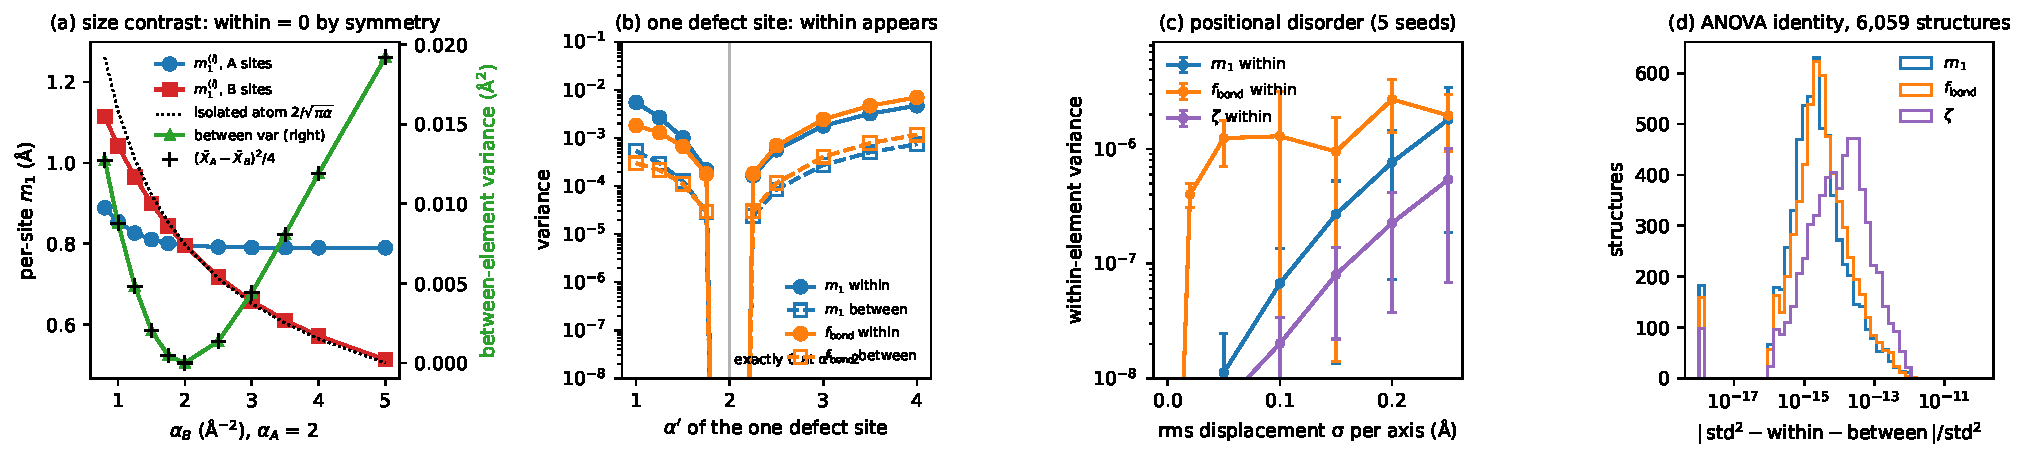
\includegraphics[width=\textwidth]{figures/si/heterogeneity_fig01_models.pdf}
\caption{Site statistics on model crystals: size contrast, one defect site,
positional disorder, and the decomposition identity over the dataset.}
\label{fig:si-het-models}
\end{figure}

\begin{figure}[htbp]
\centering
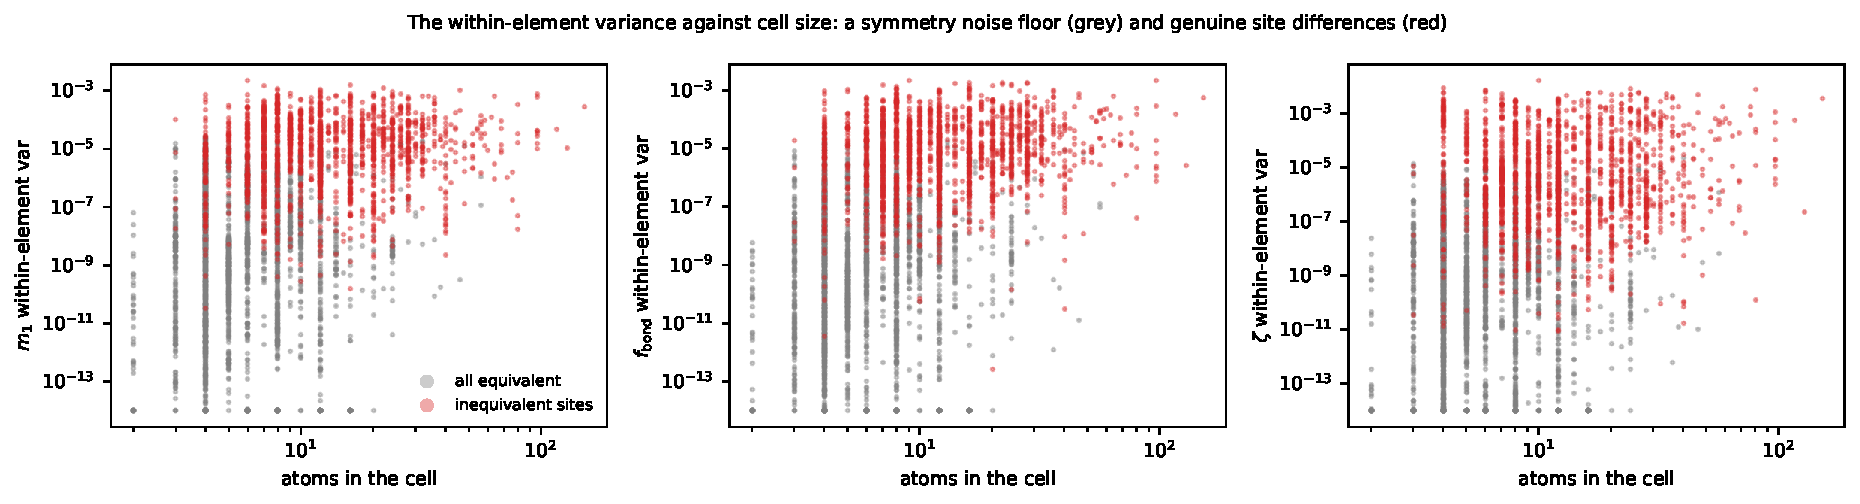
\includegraphics[width=\textwidth]{figures/si/heterogeneity_fig08_within_vs_size.pdf}
\caption{The within-element variance against cell size: the symmetry noise
floor (all sites of each element equivalent, grey) and genuine site
differences (red).}
\label{fig:si-het-floor}
\end{figure}

\begin{figure}[htbp]
\centering
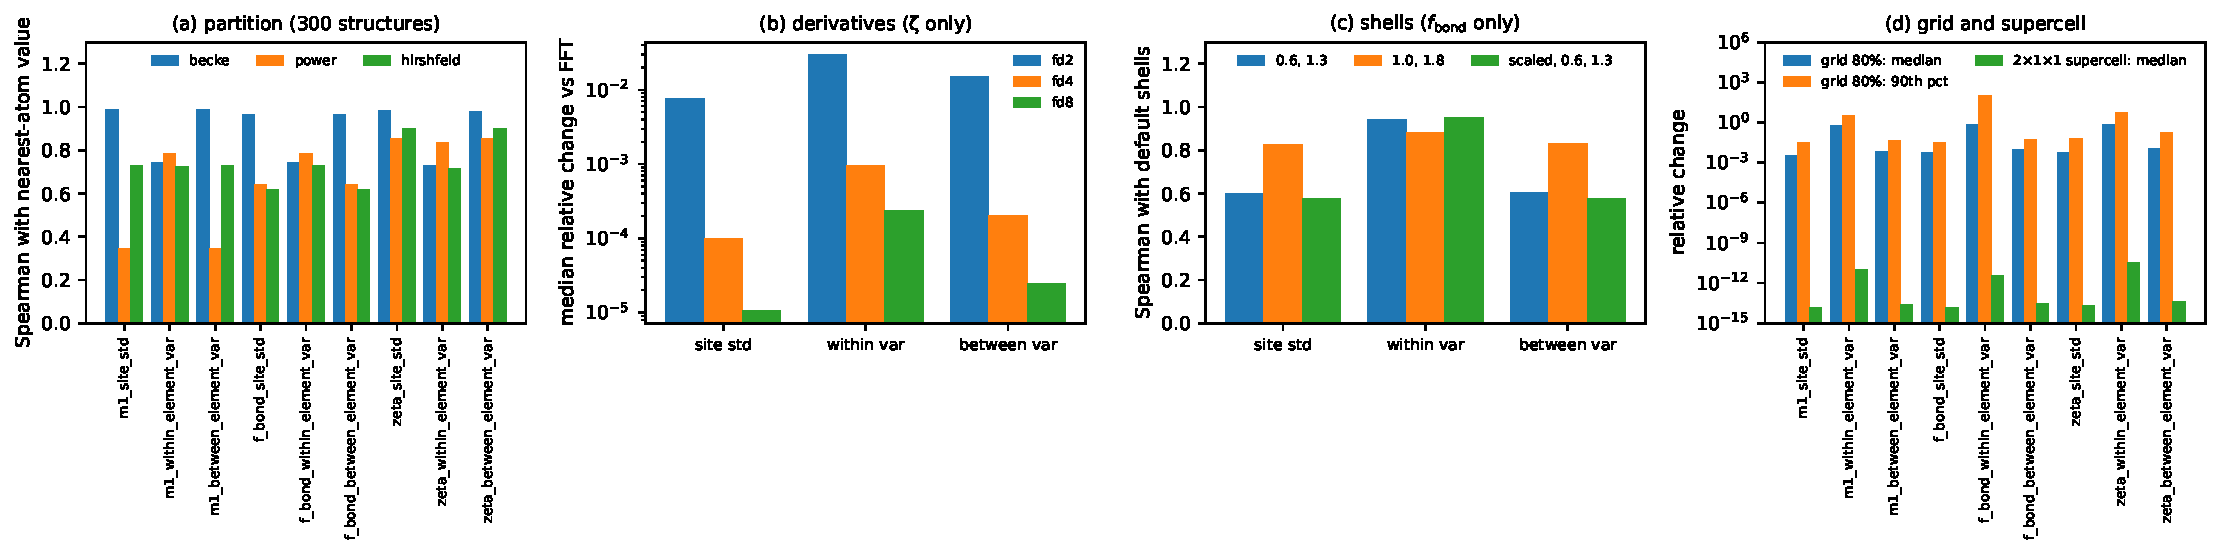
\includegraphics[width=\textwidth]{figures/si/heterogeneity_fig10_robustness.pdf}
\caption{Sensitivity of the site statistics to the partition, the derivative
scheme (\texttt{zeta} only), the shells (\texttt{f\_bond} only), the grid and a
supercell.}
\label{fig:si-het-robust}
\end{figure}

% --------------------------------------------------------------------------
\subsection{Magnetic descriptors}

For Gaussian spin densities \texttt{m1\_spin} and \texttt{sigma\_r2\_spin}
agree with their closed forms to $10^{-5}$ and \texttt{spin\_charge\_correlation}
with the exact box-integral Pearson coefficient to five decimals; in a
two-sublattice model \texttt{spin\_frustration} and \texttt{mu\_site\_std}
follow $1-|\mu_A+\mu_B|/(|\mu_A|+|\mu_B|)$ and $|\mu_A-\mu_B|/2$ exactly from
ferro- to antiferromagnetic order (Fig.~\ref{fig:si-mag-models}). The site
moments sum to the net moment to $2\times10^{-13}\,\mu_B$ on 150 real
structures. \texttt{spin\_frustration} is bounded by the voxel-level
compensation $1-M_{\mathrm{net}}/M_{\mathrm{abs}}$ and misses antiparallel
spin that the partition assigns to the sites: a ferromagnet whose interstitial
polarization cancels the net moment still gives 0.

1,679 of the 6,059 structures are magnetic ($>0.01\,\mu_B$ per atom), 1,054 of
them with a 4f element. A median 95\% of $\sum|m|$ lies inside the augmentation
spheres; 5f spin density is more extended than 4f (\texttt{m1\_spin} 0.77
against 0.64\,\AA), 4d/5d moments are small and poorly correlated with the
charge (0.44), and ionic compounds have the lowest spin--charge correlation
(oxides 0.66; Fig.~\ref{fig:si-mag-class}). \texttt{spin\_frustration} exceeds
0.5 for 83 structures, mostly rare-earth--transition-metal compounds such as
ErFe$_2$ (Er $-3.0\,\mu_B$, Fe $+1.86\,\mu_B$; Fig.~\ref{fig:si-mag-frust}). The
magnetic order is that of the calculation in its cell, not necessarily the
ground state (NiO is ferromagnetic in its 8-atom cell). ChargE3Net, as trained,
predicts the total density only, so the magnetic descriptors are not available
from predicted densities.

\begin{figure}[htbp]
\centering
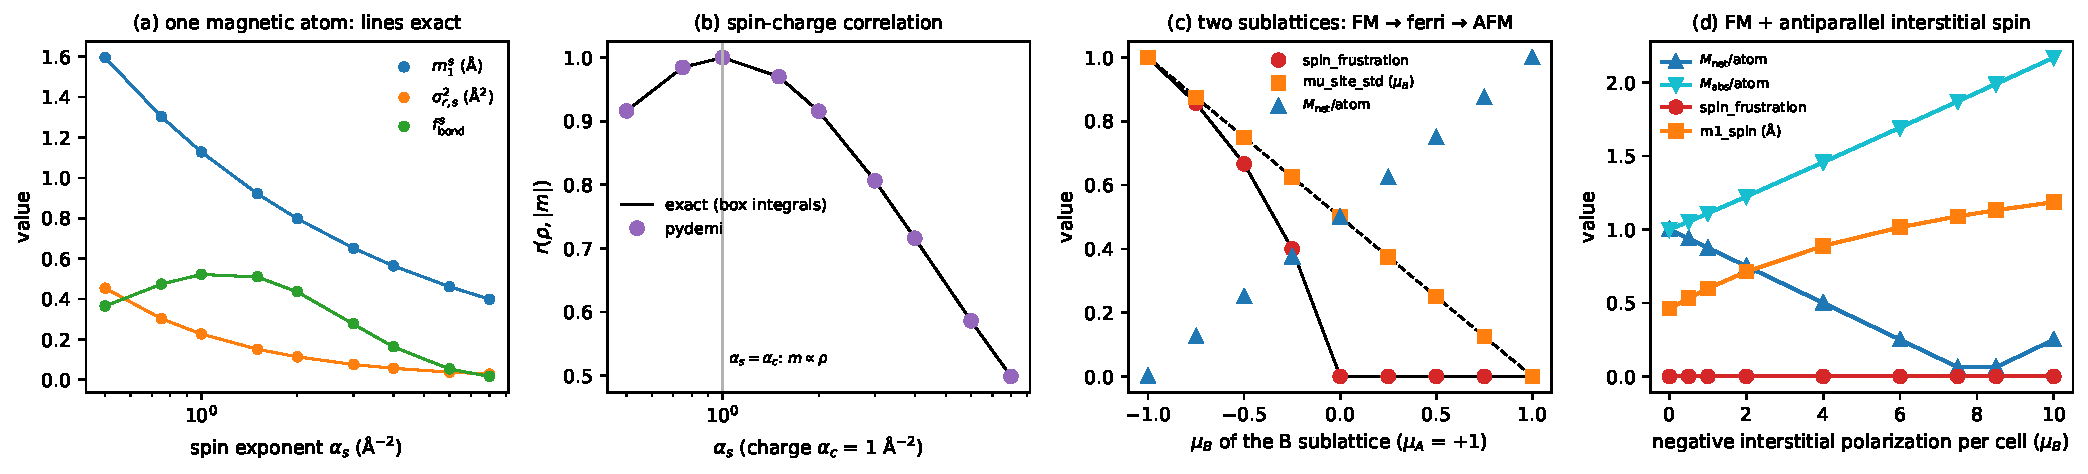
\includegraphics[width=\textwidth]{figures/si/magnetic_fig01_models.pdf}
\caption{Magnetic descriptors on model magnetization densities (lines exact).}
\label{fig:si-mag-models}
\end{figure}

\begin{figure}[htbp]
\centering
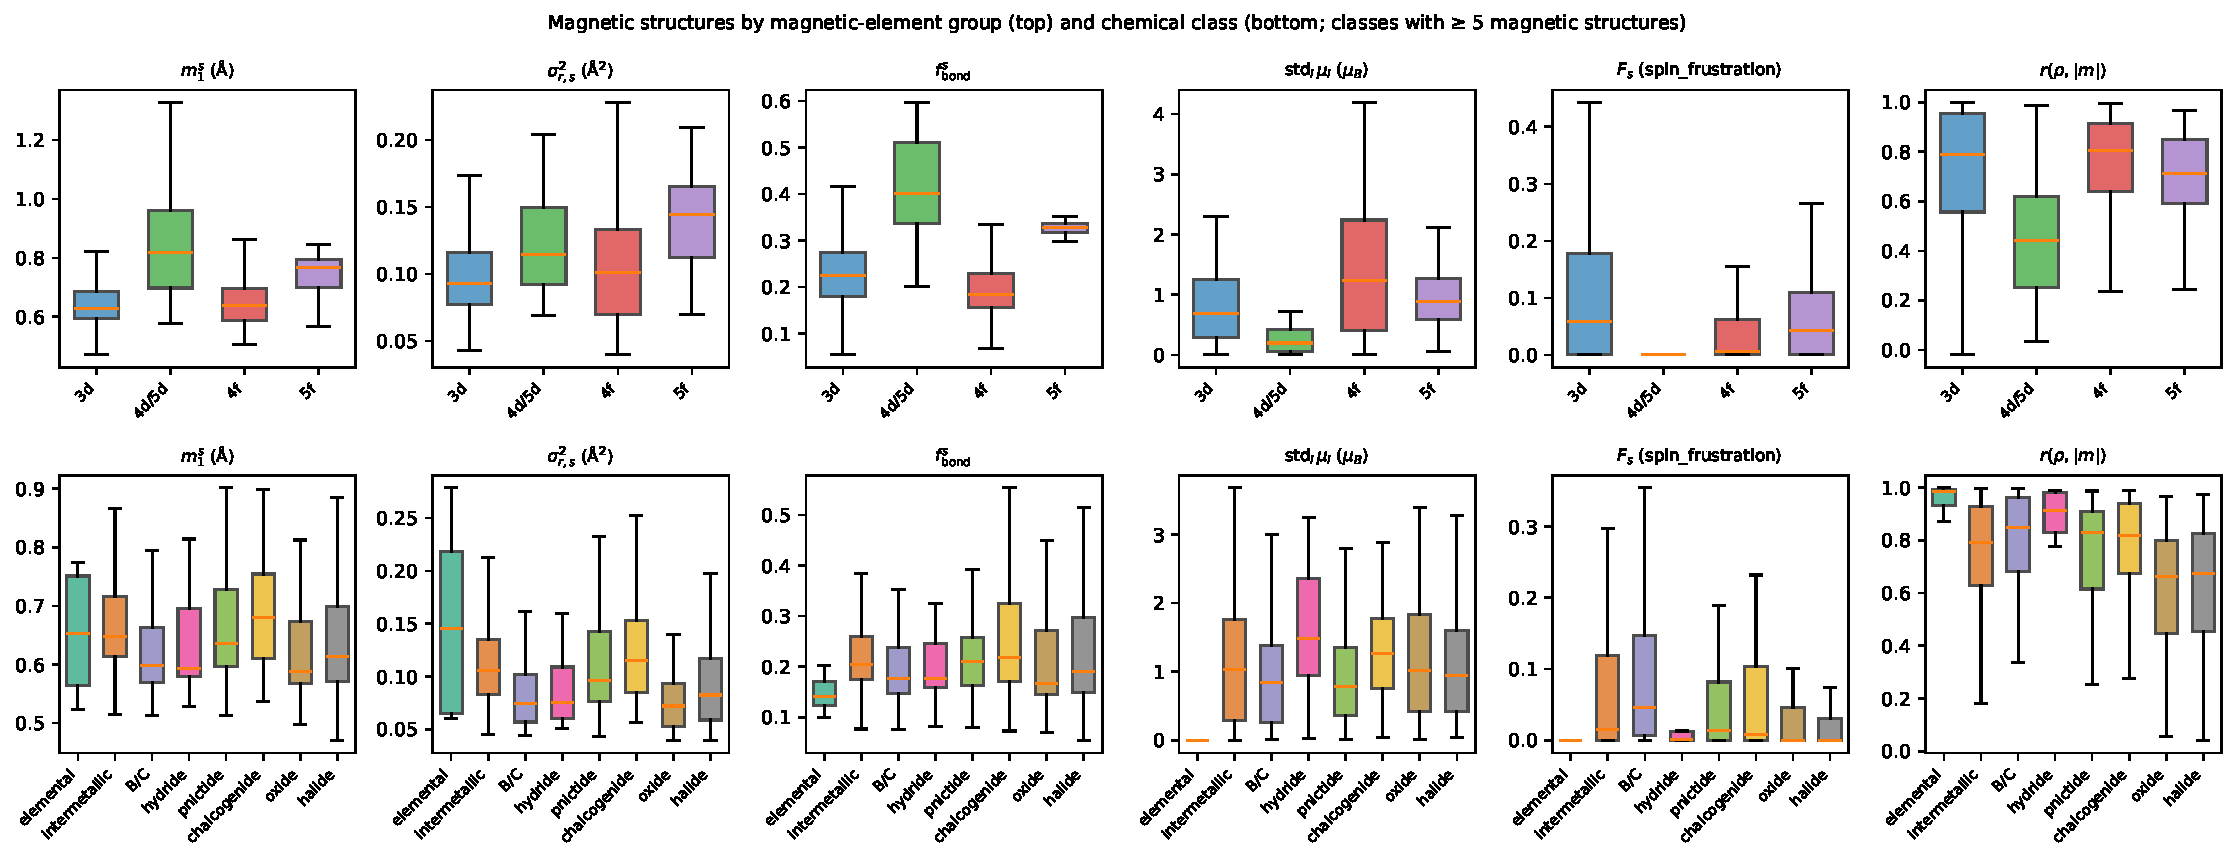
\includegraphics[width=\textwidth]{figures/si/magnetic_fig07_by_group_and_class.pdf}
\caption{Magnetic descriptors of the 1,679 magnetic structures by
magnetic-element group (top) and chemical class (bottom).}
\label{fig:si-mag-class}
\end{figure}

\begin{figure}[htbp]
\centering
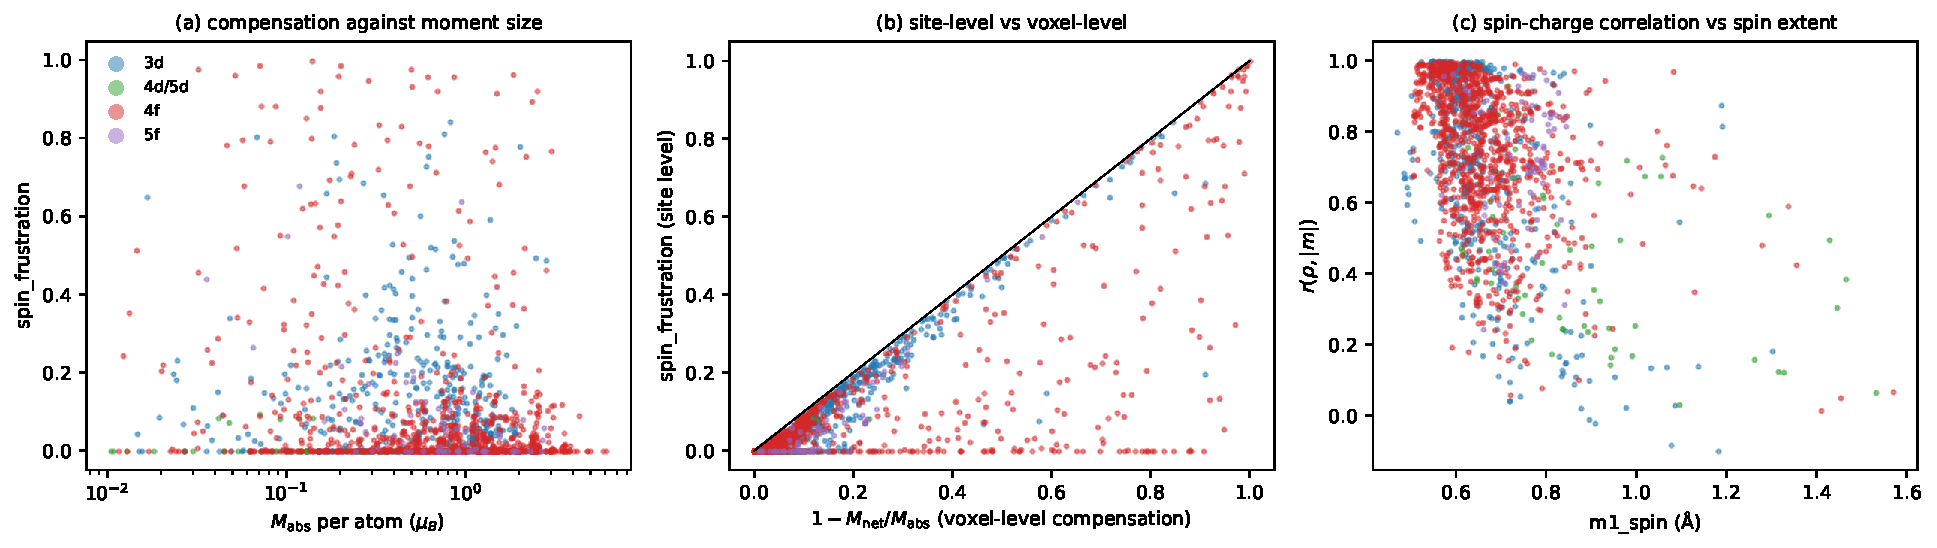
\includegraphics[width=\textwidth]{figures/si/magnetic_fig08_frustration_and_correlation.pdf}
\caption{(a) \texttt{spin\_frustration} against the moment size; (b) against
the voxel-level compensation, its upper bound; (c) the spin--charge
correlation against the extent of the spin density.}
\label{fig:si-mag-frust}
\end{figure}

% --------------------------------------------------------------------------
\subsection{Percolation and the density floor}

For a simple cubic lattice of Gaussians, the specification's test case,
\texttt{rho\_perc} equals the density at the bond midpoint and the minimum the
density at the cube centre to six digits, and a tetragonal stretch follows the
exact \texttt{perc\_anisotropy} (Fig.~\ref{fig:si-perc-models}). With the atom
off the grid points, a cubic lattice acquires a spurious anisotropy of 0.002
(0.05\,\AA\ spacing) to 0.028 (0.19\,\AA); in the dataset 95\% of the relaxed
cubic structures are below $2\times10^{-5}$.

The percolation level is the value of one voxel, the bottleneck of the best
connecting path, which can therefore be located exactly: over 200 structures,
62\% of the bottlenecks lie within 10\% of a pair midpoint, 52\% on the
shortest interatomic distance, and their median distance from the nucleus is
0.99\,$R_{\mathrm{PAW}}$ (Fig.~\ref{fig:si-perc-bottle}). The global density
minimum, by contrast, is at a nucleus in 67\% of the structures and negative in
61\%: on CHGCARs \texttt{rho\_min\_ratio} measures the pseudization dip, and the
interstitial \texttt{rho\_min\_int\_ratio} (\texttt{paw} extension) is the
physical floor. It orders the classes from elemental and intermetallic
(0.21--0.23) to halides (0.02) and falls with the electronegativity difference
(Spearman $-0.61$). The levels are high for covalent networks and metals and
low for ionic, molecular and van der Waals solids (Si 0.386, Al 0.203, NaCl
0.029\,e\,\AA$^{-3}$; NbSe$_2$ 0.44 in-plane, 0.038 across the layers;
Fig.~\ref{fig:si-perc-class}); they are not a band-gap indicator, and, being
defined along the lattice vectors, they depend on the choice of cell (a
rhombohedral primitive cell hides the layering of Ca$_2$N).

\begin{figure}[htbp]
\centering
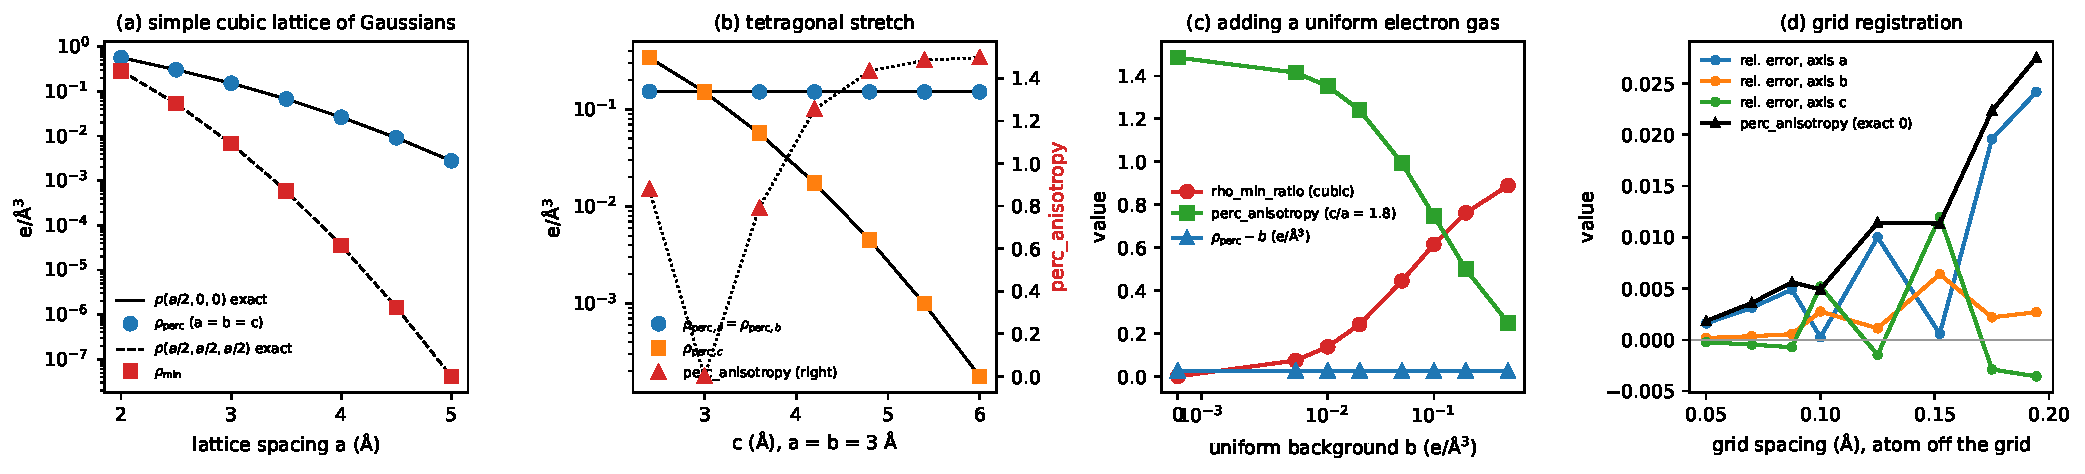
\includegraphics[width=\textwidth]{figures/si/percolation_fig01_models.pdf}
\caption{Percolation levels and the density floor on model densities, and the
effect of grid registration.}
\label{fig:si-perc-models}
\end{figure}

\begin{figure}[htbp]
\centering
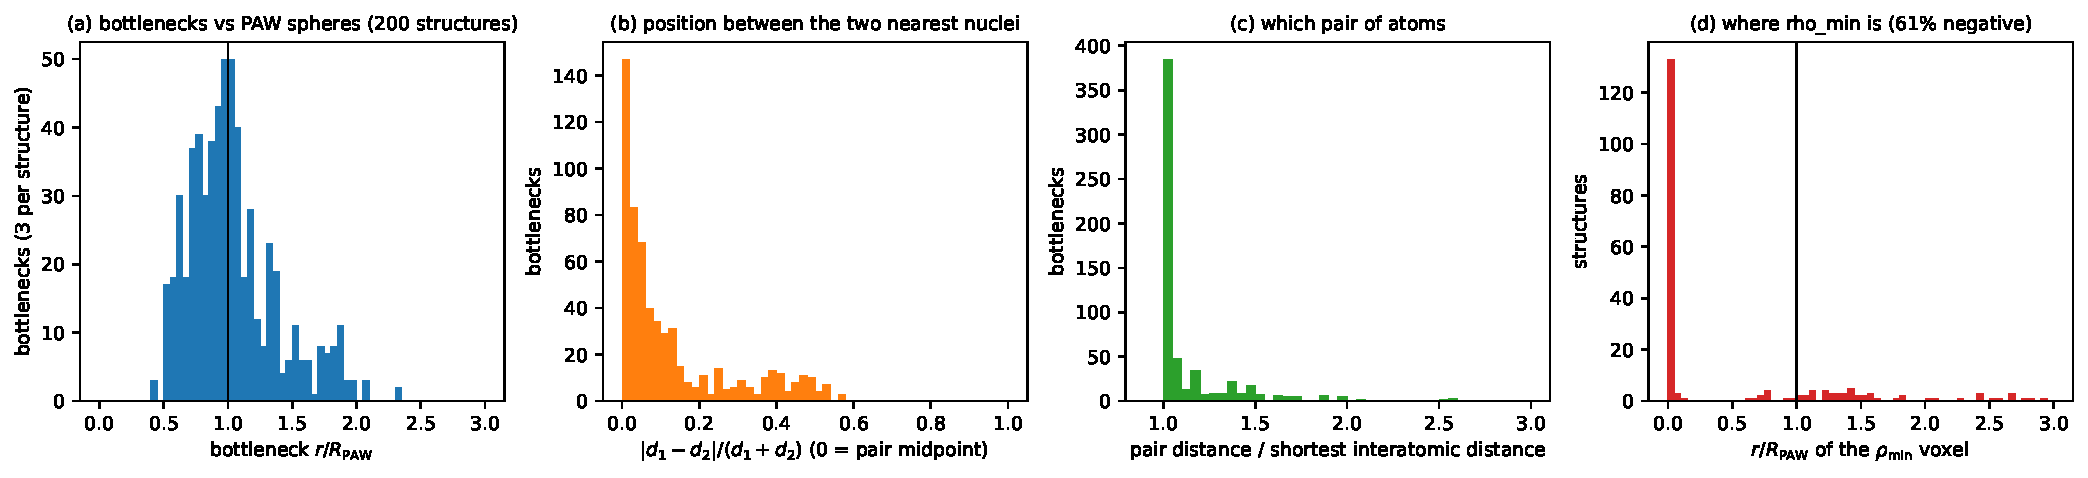
\includegraphics[width=\textwidth]{figures/si/percolation_fig03_bottlenecks.pdf}
\caption{Location of the percolation bottlenecks and of the density minimum
(200 random structures).}
\label{fig:si-perc-bottle}
\end{figure}

\begin{figure}[htbp]
\centering
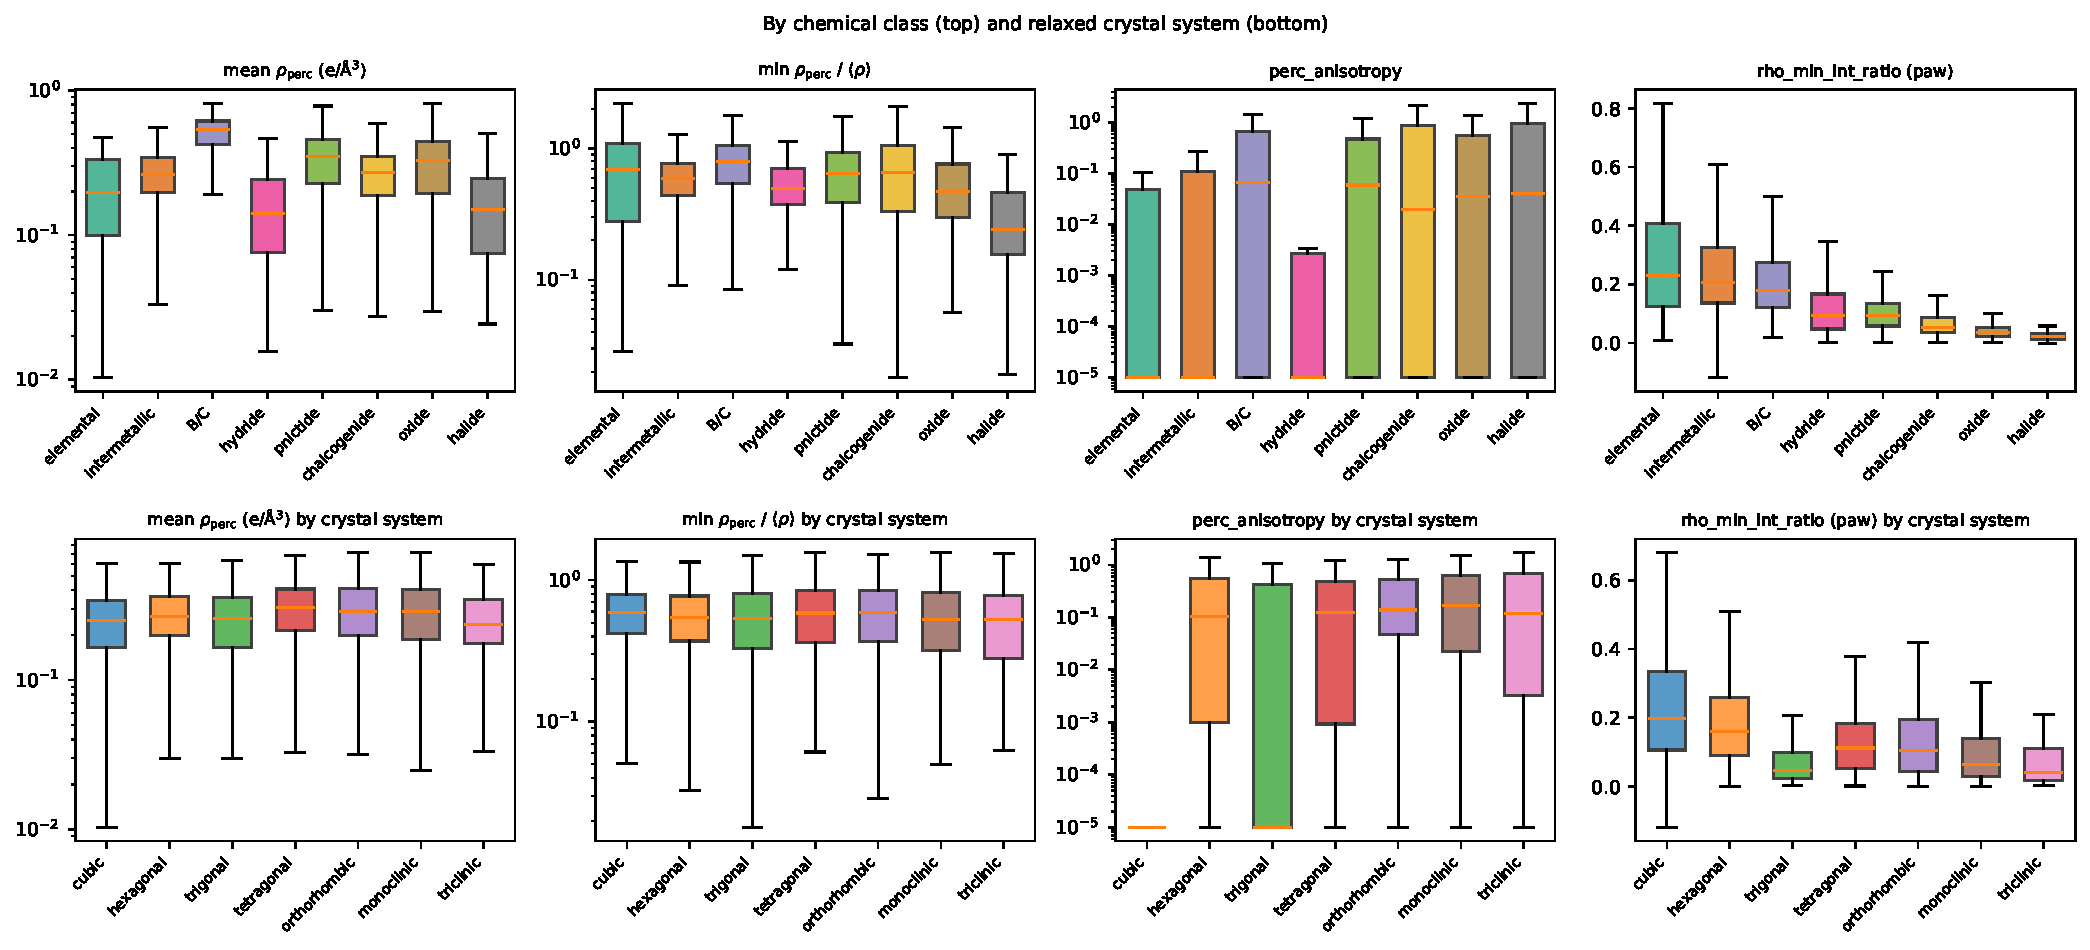
\includegraphics[width=\textwidth]{figures/si/percolation_fig05_by_class_and_system.pdf}
\caption{Percolation levels, \texttt{perc\_anisotropy} and the interstitial
density floor by chemical class (top) and crystal system (bottom).}
\label{fig:si-perc-class}
\end{figure}

% --------------------------------------------------------------------------
\subsection{Site potentials, bond midpoints and the Laplacian concentration}

\texttt{V\_spread} matches a grid-independent reciprocal-space lattice sum of
Gaussian charges to five decimals, is linear in charge transfer (14.6\,eV per
unit transfer in a rock-salt model), and is also nonzero without any charge
transfer when the atoms differ in size (Fig.~\ref{fig:si-ion-models}).
\texttt{rho\_mid\_std} matches exact midpoint densities and jumps when a bond
type crosses the census cutoff at 1.1 times the shortest distance.
\texttt{lap\_concentration} is identically $1/2$ on any periodic density,
because $\sum_k\nabla^2\rho_k=0$ on the torus (largest deviation over the
dataset $9\times10^{-16}$); the valence variant, which excludes the core shell,
matches the exact radial ratio of a Gaussian atom to $10^{-3}$ and correlates
with the bond-shell ELF (Spearman 0.85).

Without a LOCPOT, \texttt{V\_spread} uses the electronic Hartree potential, and
on the dataset it measures the contrast in valence counts between the atoms
(Spearman 0.70 with the spread of ZVAL over the sites), not charge transfer
($-0.04$ with the spread of net charges; Fig.~\ref{fig:si-ion-vspread}); with
the ionic term (\texttt{potential\_source="esp"}) the correlation with the
charge spread rises to 0.29--0.37.

\paragraph{The discontinued calibrated ionicity.} The superseded first build
of pydemi contained a calibrated ionicity, $\sigma(b_0+\sum_j b_jz_j)$ of the
standardized features $f_{\mathrm{int}}/\mathrm{lnf}$ and \texttt{V\_spread}
fitted to Phillips' ionicities, and its difference from the Pauling ionicity.
Reconstructed on the current descriptors and fitted to the 62 Phillips
compounds in the dataset, it reaches a leave-one-out RMSE of 0.189 on the 32
verified targets, no better than a sigmoid of the Pauling ionicity alone
(0.184), and 0.242 on all 62 (Pauling 0.192); it over-predicts the Zn and Cd
chalcogenides (0.96--1.00 against 0.61--0.70) because of their $d^{10}$ PAW
valence, and extrapolates to a median of 0.83 for intermetallics
(Fig.~\ref{fig:si-ion-cal}). It is therefore not part of the current release.

\begin{figure}[htbp]
\centering
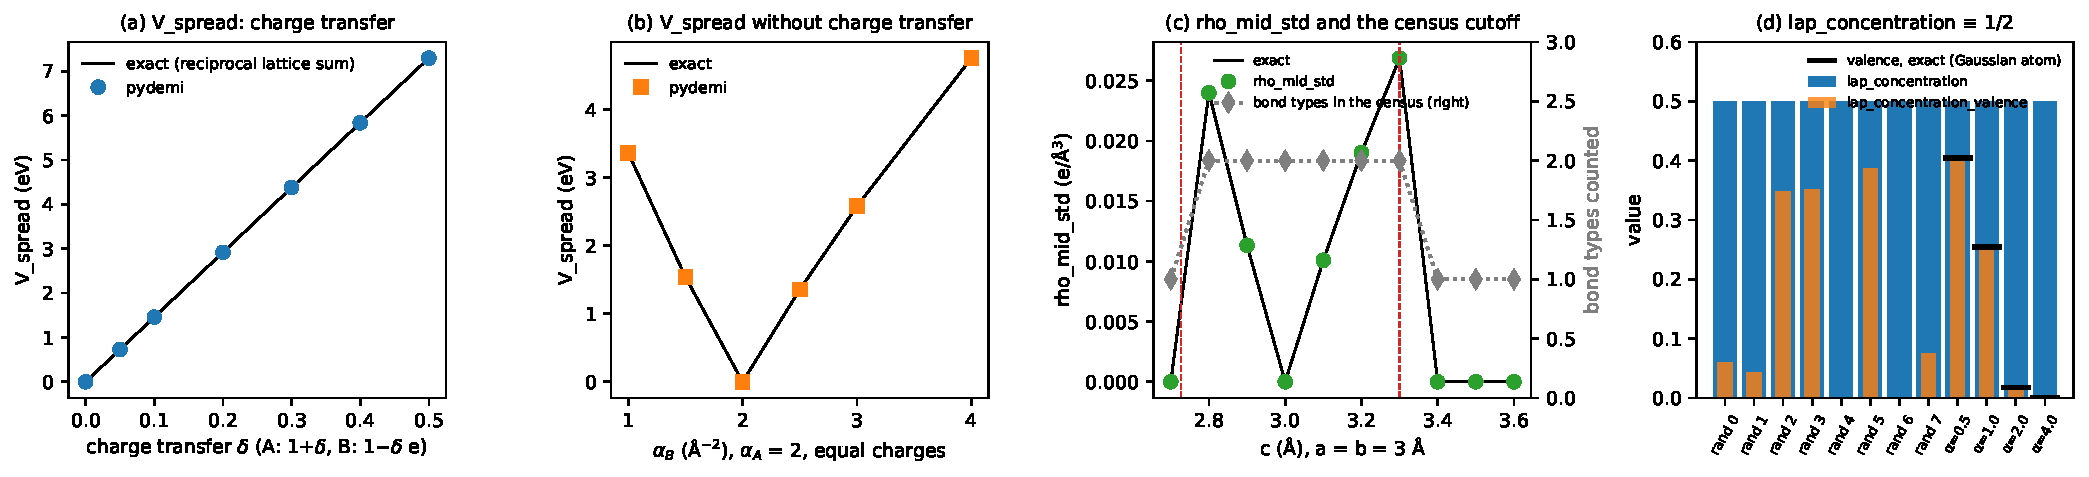
\includegraphics[width=\textwidth]{figures/si/ionicity_fig01_models.pdf}
\caption{\texttt{V\_spread}, \texttt{rho\_mid\_std} and
\texttt{lap\_concentration} on model densities (lines exact).}
\label{fig:si-ion-models}
\end{figure}

\begin{figure}[htbp]
\centering
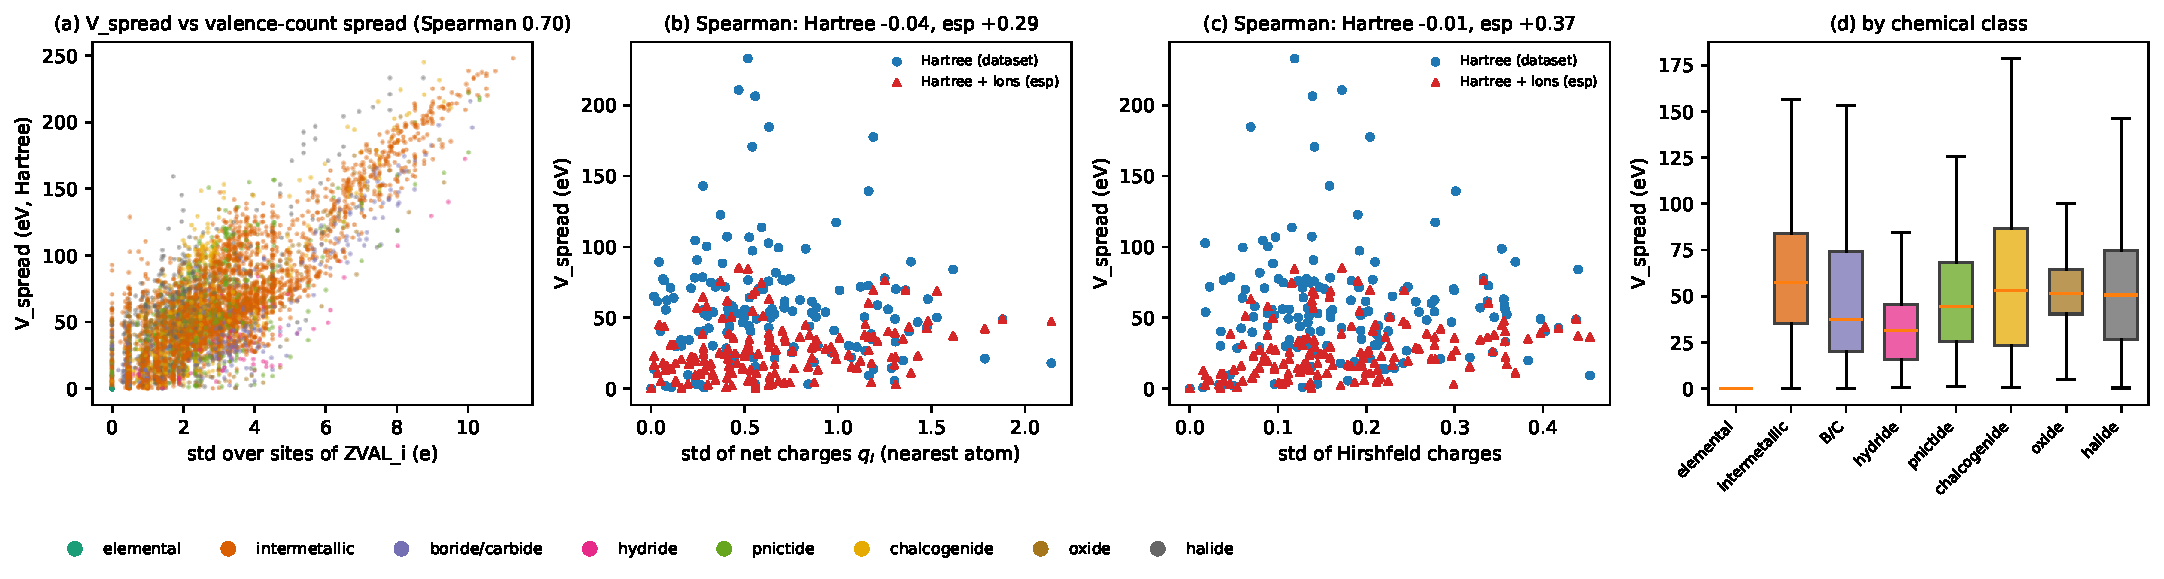
\includegraphics[width=\textwidth]{figures/si/ionicity_fig02_V_spread.pdf}
\caption{What the Hartree \texttt{V\_spread} measures: valence-count contrast
(a) rather than charge transfer (b, c); (d) by class.}
\label{fig:si-ion-vspread}
\end{figure}

\begin{figure}[htbp]
\centering
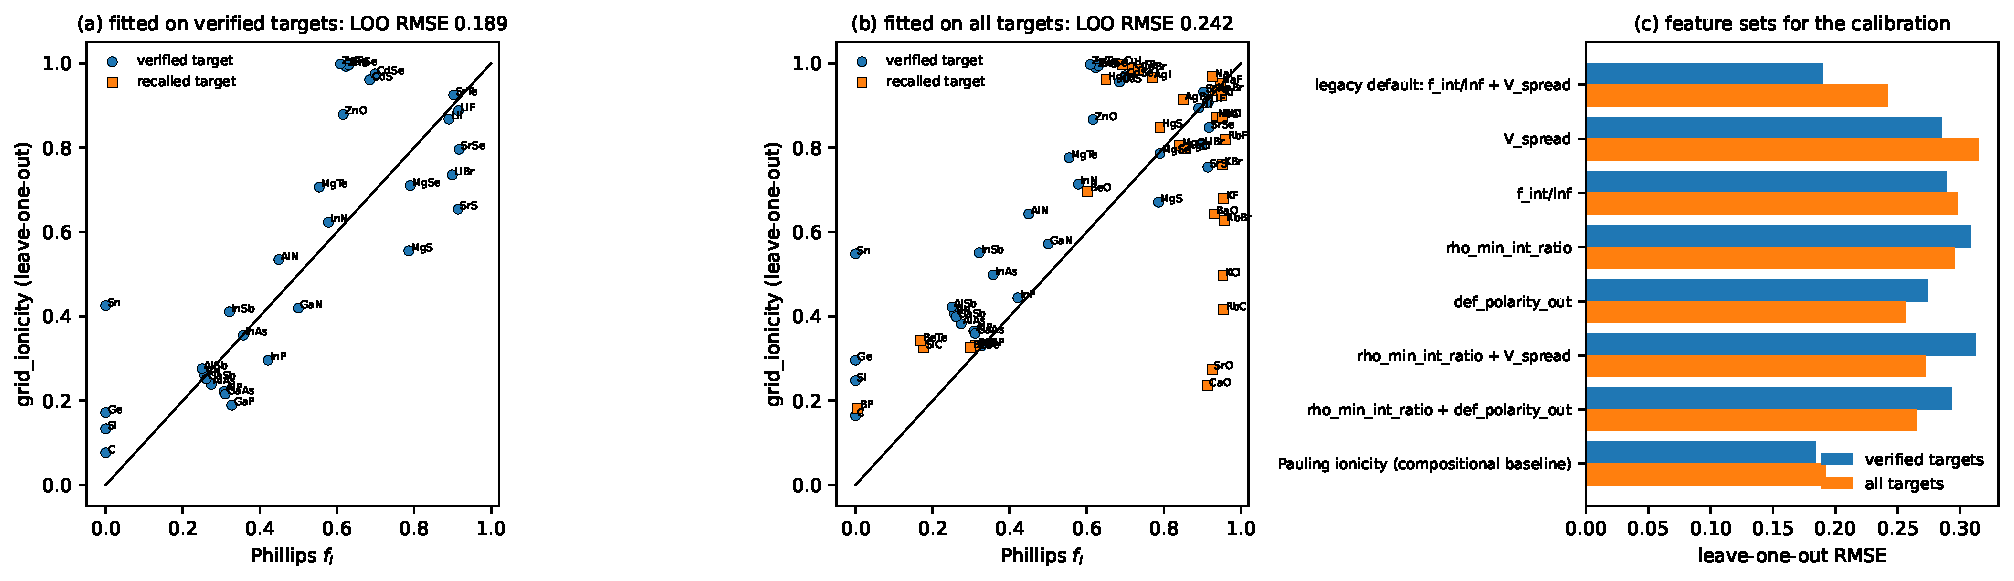
\includegraphics[width=\textwidth]{figures/si/ionicity_fig05_calibration.pdf}
\caption{The reconstructed calibrated ionicity: leave-one-out predictions
against Phillips' ionicities and the error of alternative feature sets,
including the compositional Pauling baseline.}
\label{fig:si-ion-cal}
\end{figure}

% ==========================================================================
\section{Validation details}
\label{sec:si-validation}

% To be written with main-text Section 5: the 876 tests grouped by kind
% (analytic densities with closed forms, exact identities, invariance harness
% over every descriptor, reference data, I/O and unit conversions, regression
% tests), with the tolerances achieved.

% ==========================================================================
\section{Dataset and DFT settings}
\label{sec:si-dataset}

The dataset contains 6,059 VASP charge densities of 87 elements, named
\texttt{<formula>\_<space group>}: 86 elemental solids, 3,195 intermetallics,
354 borides/carbides, 80 hydrides, 653 pnictides, 548 chalcogenides, 607
oxides and 536 halides. Each run folder holds the CHGCAR; 4,901 also hold the
OUTCAR, from which the settings in Table~\ref{tab:si-dft} were parsed. All
parsed runs share one protocol: PBE with one PAW dataset per element, a
500\,eV cutoff, collinear spin polarization, the tetrahedron method and an
automatic $k$-mesh of spacing at most about 0.1\,\AA$^{-1}$, as single-point
calculations (\texttt{NSW = 0}) on the supplied structures. The relaxation that
produced these structures is not part of the dataset; for 373 structures the
crystal system of the relaxed structure differs from the space group in the
run name. 221 of the parsed runs (4.5\%, 133 of them intermetallics) stopped
at \texttt{NELM = 200} without reaching \texttt{EDIFF}; they are kept in the
analysis and listed in \texttt{paper/analysis/out/dft\_settings.csv}. The 1,158 runs without an OUTCAR are assumed to
follow the same protocol; their valence counts and PAW radii come from a
per-element table built from the other runs, which use one PAW dataset per
element throughout (main text, Section~4.3).

\begin{table}[htbp]
\centering
\caption{DFT settings of the dataset, parsed from the 4901 runs that include their OUTCAR (\texttt{paper/analysis/j\_dft\_settings.py}). The other 1158 runs have only the CHGCAR.}
\label{tab:si-dft}
\small
\begin{tabular}{p{4cm}p{10.5cm}}
\toprule
VASP version & 5.3.3 (4663), 5.4.4 (238) \\
Exchange-correlation & PBE (\texttt{LEXCH = PE}) in all runs; no meta-GGA, no $+U$, no van der Waals correction \\
PAW datasets & 87 PAW\_PBE datasets, one per element throughout \\
Plane-wave cutoff & \texttt{ENCUT} = 500 eV, \texttt{PREC = Accurate} (all runs) \\
Spin & collinear spin-polarized (\texttt{ISPIN = 2}) in all runs; initial moments not recorded in the OUTCAR \\
Electronic convergence & \texttt{EDIFF} = $10^{-6}$ eV, \texttt{NELM} = 200; 221 runs (4.5\%) stopped before reaching \texttt{EDIFF} \\
Ionic steps & none (\texttt{NSW = 0}, \texttt{IBRION = -1}): single-point calculations \\
Brillouin-zone integration & tetrahedron method with Bl\"ochl corrections (\texttt{ISMEAR = -5}) in 4898 runs; Gaussian, 0.03 eV in 3 \\
$k$-points & automatic mesh; largest spacing $|\mathbf b_i|/N_i$ median 0.098\,\AA$^{-1}$ (5th--95th percentile 0.094--0.100, $2\pi$ included) \\
Projection & reciprocal space (\texttt{LREAL = F}) in 4461 runs, \texttt{Auto} in 440 \\
Output & CHGCAR (\texttt{LCHARG = T}); ELF written (\texttt{LELF = T}), but the ELFCAR is distributed for only 86 runs; no LOCPOT (\texttt{LVTOT = F}), no AECCAR (\texttt{LAECHG = F}) \\
\bottomrule
\end{tabular}
\end{table}


% ==========================================================================
\section{Machine-learning details}
\label{sec:si-ml}

% To be written with main-text Section 7: ChargE3Net architecture and training
% on the dataset (split, grids, probe sampling), fine-tuning from the Materials
% Project checkpoint, probe versus full-grid NMAPE for the three models,
% the descriptor-level DFT-vs-ML table for every descriptor, and the failure
% cases (f-electron compounds).

% \bibliographystyle{unsrt}   % enable when the SI cites references
% \bibliography{references}

\end{document}
